\chapter{Thesis Contributions}
The general contribution of the thesis is a safety-critical design approach that employs formal methods at various stages of software development such as requirements specification and software design, and a power-efficient mapping of software to hardware while satisfying timing and reliability of the software in a distributed environment. It satisfies the research goals explained in Subsection~\ref{research_challenges} via the following contributions: a requirements specification language tailored to embedded systems~\cite{Mahmud2015ReSA:Systems}\cite{resatool}, formal analysis of the specifications~\cite{resatool}\cite{Mahmud2017SpecificationLogic} via formal and knowledge-based methods, formal analysis of large-scale Simulink models~\cite{Filipovikj2018SimppaalModels} and efficient mapping of software to hardware in the context of distributed architecture~\cite{Mahmud5222}\cite{Mahmud2019Power-awareOptimization} via integer-linear programming and metaheuristics. 

Figure~\ref{fig_workflow} illustrates the workflow of an embedded software development that make of use our contributions. The workflow is contextualized in the automotive software development where Simulink, EAST-ADL and AUTOSAR architectural language are used. 
\begin{figure}[h]
	\centering
	\ifpdf
	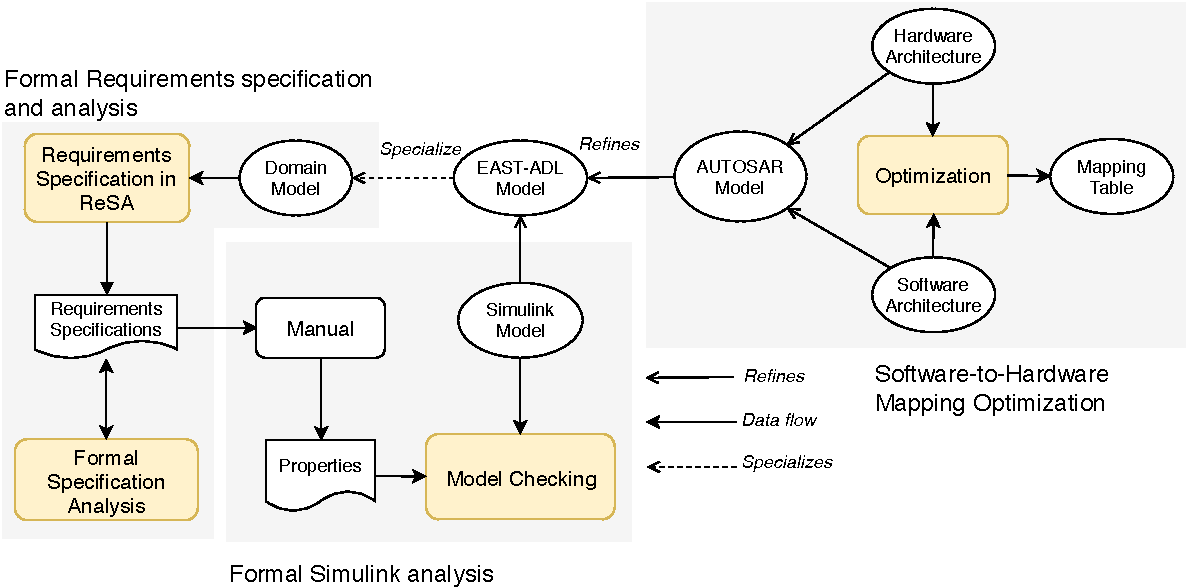
\includegraphics[width=\linewidth]{images/workflow}
	\else
	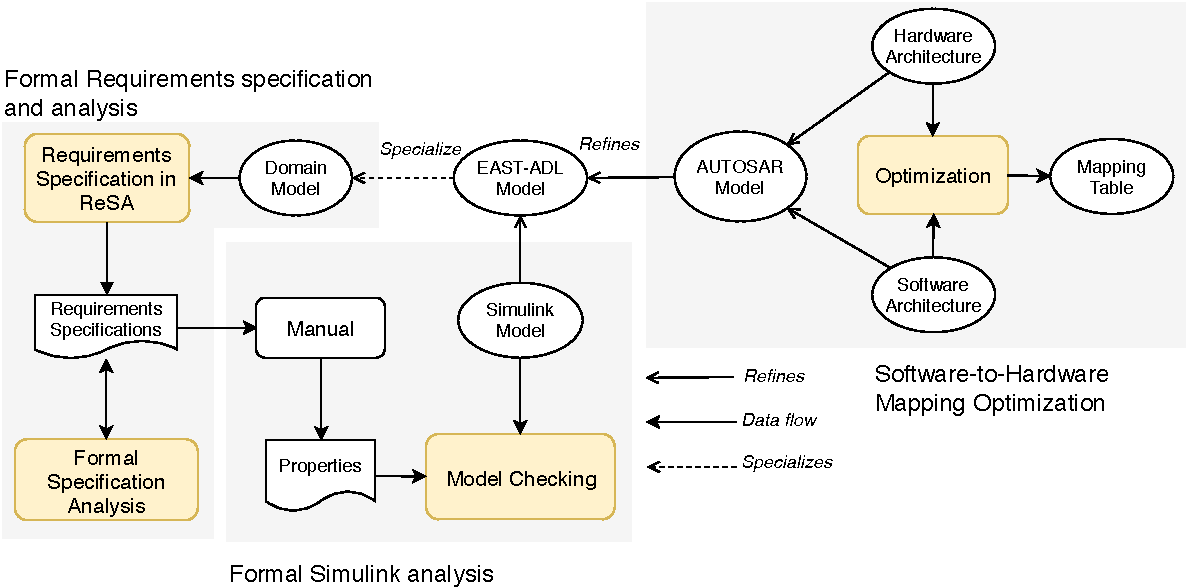
\includegraphics[width=.8\linewidth]{images/workflow.eps}
	\fi
	\caption{Thesis contributions workflow.} 
	\label{fig_workflow}
\end{figure}

Initially the textual requirements are specified in our domain-specific language ReSA, which is a constrained natural language that is specific to embedded systems. The ReSA editor supports content completion as it is connected to a system model, which is generic. However, If the ReSA editor is required to be integrated into  domain-specific architectural models, the latter specializes the ReSA concepts, hence enabling domain-specific access. To check the consistency, the ReSA specifications are translated into formal specifications such as Boolean and description logic, subsequently, analyzed via SAT solver and inference engine (or reasoner), respectively.

After the quality of the specifications are improved, i.e., become unambiguous,  comprehensible, consistent, they can be used in the verification of behavioral software designs, thus reducing later errors detection and maintenance. In this work, we consider the behavior models that are designed in Simulink, which is one of the most widely used environment for modeling, simulation and analysis of embedded systems. In order to rigorously analyze a Simulink model, it is transformed into a formal model, subsequently, the latter is analyzed via statistical model checking against properties initially expressed in ReSA, and manually translated into the query (properties) language of the model checker.

The Simulink model, at the architectural level, is represented by a system architecture, which consists of software and hardware architectures. Note that, the relation between the Simulink model and the system architecture is by refinement, and is mostly manual, which is also the case in this work. The software architecture complements the behavioral model with computational resource specifications, e.g., CPU, memory, and other system critical resource specifications, e.g., power consumption. In this regard, the software to hardware mapping can be efficiently made via optimization techniques. Our proposed optimization techniques incorporate the timing requirements of the software. Although the input model to the optimization is an AUTOSAR model, the approach can be applied to any component-based embedded software development through minor modification. 

In the next subsections, we discuss the contributions in detail.
\section{ReSA - a Constrained Requirements Specification Language of Embedded Systems}\label{rc_resa}
The language is designed to improve comprehensibility and reduce ambiguity of embedded systems specifications. It is a constrained natural language on both syntax and semantic levels. It employs embedded system concepts such as System, Parameter, Device, State, Mode, Entity, etc, to identify words/phrases of specification and relations between between instance of the concepts to enforce semantics (or interpretations) at the syntactic level, e.g., the fact is a system can be activated, but not parameters, a user is notified, but not a system. 

The syntactic rules allow construction of valid statements, reduce ambiguity and improve readability. The valid instantiations of the ReSA language are sentencial forms (or requirements boilerplates), as shown in Table~\ref{tbl_boilerplates}. The specification is finalized by filling the variable elements of the boilerpaltes, which the syntax {\small Word|"Words"}$:Type$, e.g., "ASL speed control"$:parameter$, ASL$:system$, as illustrated by examples in Tables~\ref{fig_resa_examples}. In the ReSA editor, the boilerplates can be created for reuse.
\subsection{Syntax}
\begin{table}[h]\small
	\begin{tabular}{@{}lp{0.75\textwidth}@{}}
		\toprule
		Boilerplate & Description \\ \midrule
		Simple & instantiates a simple statement, e,g., \texttt{Simple := System Verb within Quantity TimeUnit.} \\
		Compound & instantiates a compound statement, e.g., \texttt{Compound := Simple and/or {Simple}+} \\
		Complex & instantiates complex statement, and is constructed from Simple and a subordinating conjunction, such as when, while, until, e.g., \texttt{Complex := if Simple, Simple} \\
		Nested-Complex & instantiates nested-complex statements, and is constructed from independent clause and complex boilerplate(s), e.g., \texttt{Ncomplex := after Simple, Complex.} \\
		Conditional & instantiates conditional statements including if, if-else, if-else-if \\ \bottomrule
	\end{tabular}
\caption{Requirements boilerplates syntax.}\label{tbl_boilerplates}
\end{table}

\begin{table}[h]
\noindent\fbox{
\small
	\begin{tabular}{lp{.9\textwidth}}
		R1 & ASL:system shall send "the driver"\textit{:user} notification:status every 200ms. \\[6pt]
		R2 &\begin{tabular}[t]{@{}l@{}}if driver selects ``ASL speed control''\textit{:mode} and\\
			\hspace{0.5cm}(vehicle is in ``pre-running'' mode or
			vehicle is in ``running'' mode)\\ then\\
			\hspace{0.5cm}ASL:system shall be enabled within 200ms and\\
			\hspace{0.5cm}``ASL enabled''\textit{:status} shall be presented to ``the driver''\textit{:user} \\ endif\end{tabular} \\[6pt]
		R3 & After ASL:system is enabled, if IncButton\textit{:inDevice} is pressed, ASL:system shall be activated.\\[6pt]
		R4 &if driver selects ``ASL speed control''\textit{:mode}
			then 
	    	ASL\textit{:system} shall be disabled.
	\end{tabular}
}%
\caption{Examples of requirments specified in ReSA.}\label{fig_resa_examples}
\end{table}

\section{Formal Analysis of ReSA Specifications}\label{rc_resaanalysis}
The ReSA specifications are transformed into Boolean and propositional logics to conduct rigorous analysis besides syntax and type checking such as consistency checking. The Boolean expressions are check for consistency via a SAT solver, and the description-logic specifications via an ontology inference engine. 

\subsection{SAT-based Analysis}
The specifications are translated into Boolean expressions, subsequently, an SMT solver is employed to check the consistency of the specifications. The analysis is scalable as the SAT solving is scalable to thousands of propositional variables, though shallow since the details of each clause in the specifications are abstracted away by a propositional variable. Thus, advanced analysis is not possible or suitable using the SAT approach.%, e.g., the clauses ``ASL is activated'' and "ASL is deactivated" are represented by two variables and does not cosider the lexical relation between the `activated'' and ``deactivated'' words, which in fact are antonyms. Moreover, temporal analysis is not suitable or intractable. 
\begin{definition}[Inconsistency of specifications]
	Let $\Phi = \{\Phi_1, \Phi_2,\dots,\Phi_n\}$ is the set of requirements specifications after translating ReSA specifications into Boolean expressions, where  $\Phi\in N$ is a Boolean formula and denotes a requirement specification. Thus, the set Boolean expressions $\Phi$ is inconsistent if the expression $\Phi_1 \land \Phi_2 \land\dots\land \Phi_n \Rightarrow false$ holds, that is, there exists at least one expression that cannot be satisfied, i.e., $\Phi_i\models false$.
\end{definition}
\begin{example}
Figure~\ref{fig_z3} illustrates the translation of the ReSA specifications R1, R2, R3, R4, into Boolean expressions, encoded as Z3 (or SMT-LIB) format. %The propositional variables $p_1-p_{11}$ represent the clauses of R1-R4, in order of occurence, that is $p_1$ represents ``ASL:system shall send "the driver"\textit{:user} notification:status every 200ms.'', $p_2$ ``driver selects ``ASL speed control''\textit{:mode}'', etc. Some clauses are resolved for negation and opposite words, e.g., the fact that ``enabled'' is opposite of ``disabled'' redners $p_5=p_7\neq p_{11}$. Alos, the user has to assert a condition holds before evaluating for consistency, e.g., condition of R2 holds, results the assertion at line 30. 
The expressions are fed into the Z3 solver, which returns the unsat-core feedback "unsat (R1, R2 R1\_Assertion)". The unsat-core shows that R2, R4 and the R2 assertion are the source of the inconsistency. Note that, Z3 only tracks labeled assertions.
\end{example}
%To illustrated this point, let us localize the inconsistency using the example at the propositional level. Obviously, we see from the feedback that $p2$ must evaluate to true for the assertion R2\_assertion to hold (line 30), which means $p_5=p_6=true$ for R2 to  hold, following the logical implication rule. Since $p_5\neq p_{11}$, $p_{11}=false$, which means R4 does not hold. Consequently, satisfying our definition of inconsistency. 
\begin{figure}[h]
	\centering
	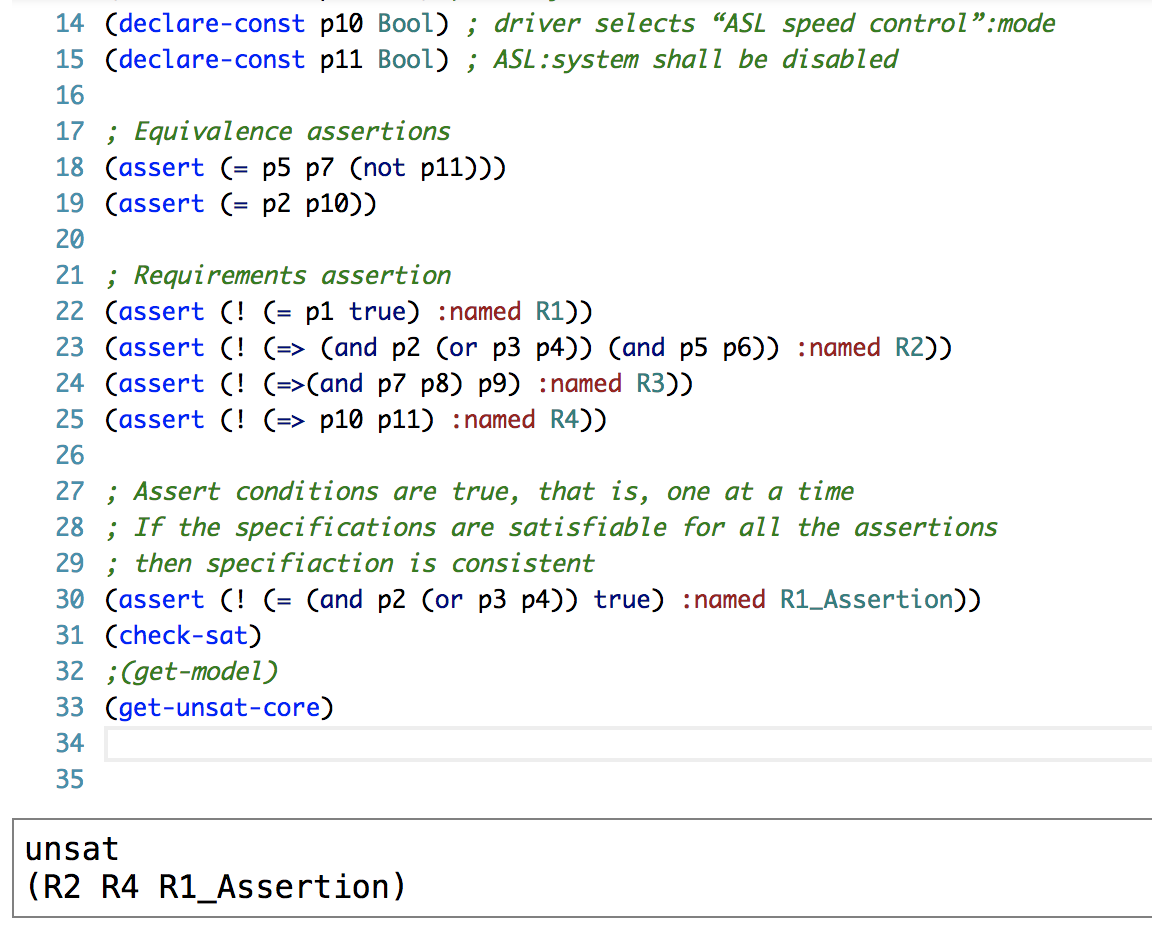
\includegraphics[width=0.7\linewidth]{images/z3}
	\caption{The ReSA specifications R1- R4 encoded as Z3 format, and the unsat-core feedback from the Z3 solver, to localize source of the inconsistency.}
	\label{fig_z3}
\end{figure}

The SAT-based analysis, although, easy and scalable, does not enable rigorously analysis at the lexical level, due to lack of adequate semantic relations defined between words/phrases. This is due to the fact that, the propositional variables abstract away these details. In the next subsection, we employ ontology-based specification to capture the syntax, and interpretation of the specifications based on the \textit{event-based} linguistic approach~\cite{Mahmud2017SpecificationLogic}.

\subsection{Ontology-based Analysis}
The event-based semantics, which is based on the first-order logic, uses an existentially quantified events to relate words/phrases (or arguments of predicate) , clauses, adjuncts of a sentence~\cite{Mahmud2017SpecificationLogic}, e.g., the clause ``ASL:system shall limit ``vehicle speed'':parameter'' is represented as $\exists e$[limiting($e$) \& Agent(ASL) \& Recipient(vehicle speed)], where Agent and Recipient are known as \textit{thematic} roles, which define the semantic roles of the arguments in the clause.  Some of the thematic roles applied in this work are shown in Table~\ref{tbl_thematic_roles}. Since the requirement specifications entail technical words/phrase, the thematic roles of these arguments are not obvious, so we define relations between the embedded system concepts shown in Tables~\ref{tbl_resa_concepts} to the thematic roles define in Table~\ref{tbl_thematic_roles}, e.g., any instance of System or User is Agent, similarly instances of Parameter is Recipient, etc. In this way, the interpretation of the clauses become domain-specific.
\begin{table}[h]\small
	\begin{tabular}{@{}lp{0.75\textwidth}@{}}
		\toprule
		Thematic Role & Description \\ \midrule
		Agent & initiates and carries out an action, and exists independently of the action. \\
		Attribute & is the property of an entity. \\
		Patient & undergoes state changes and exists independently of the action. \\
		Theme & similar to Patient, but doesn't undergo state changes. \\
		Recipient & is the destination of an action. \\
		Instrument & is used by an agent to cause an action, and exists independently of the action. \\ \bottomrule
	\end{tabular}
\caption{Thematic roles.}\label{tbl_thematic_roles}
\end{table}

A complex requirements specification can be constructed via the composition of events, e.g., ``after ASL button is pressed, ASL shall limit ``vehicle speed'' is represented as $\exists e_1$[pressing($e1$)\&Recipient(ASL button)\& $\exists e_2$[activating($e_2$)\&Agent(ASL)\&Recipient(vehicle speed)]\& after($e_1,e_2$)].

Following the event-based semantics, the ReSA specifications are translated into description logic as ontology, which is a knowledge representation approach frequently used in artificial intelligence, and information system, e.g., the world-wide web. The ontology contains terminological assertions and concrete assertions, respectively assert, the logical structure of sentences according to the event-based semantics, and the requirements specifications, such as the types, thematic roles of words/phrases, respectively. Figure~\ref{fig_ontology} the concepts, relations and instances of the requirements specifications ontology.
\begin{figure}[h] 
	\centering
	\subfloat[Concepts.\label{fig_continuous}]{% 
		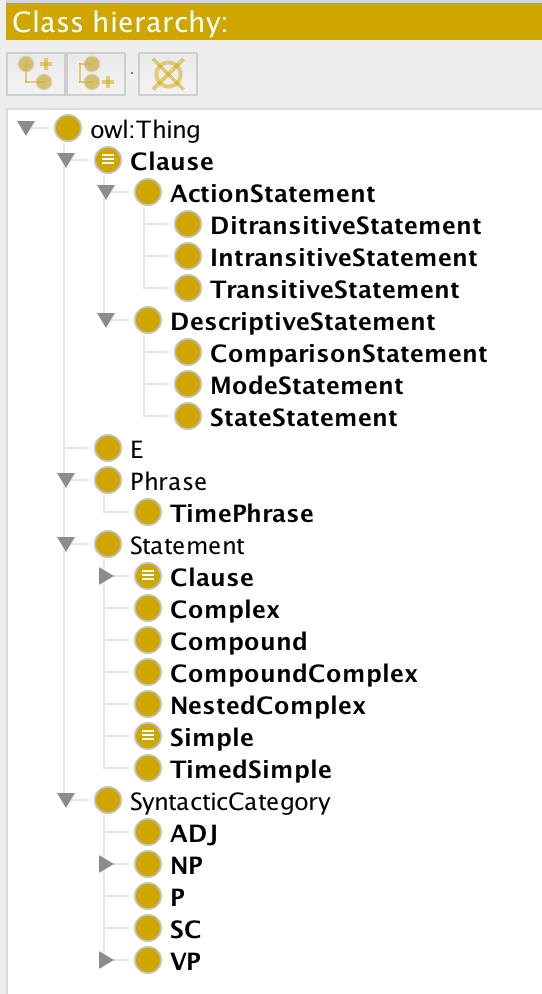
\includegraphics[width=0.3\textwidth]{images/ro_concepts}
	} \hfill
	\subfloat[Object properties.\label{fig_discrete}]{% 
		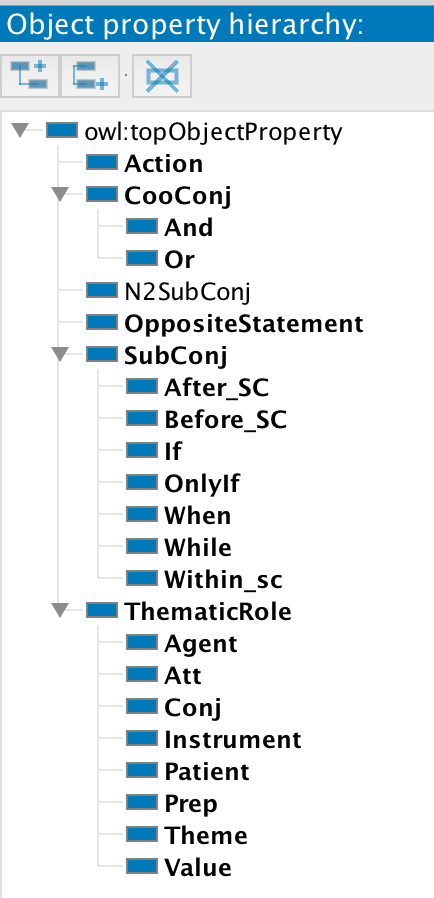
\includegraphics[width=0.3\textwidth]{images/ro_objects} 
	} 
\hfill
\subfloat[Individuals.\label{fig_discrete}]{% 
	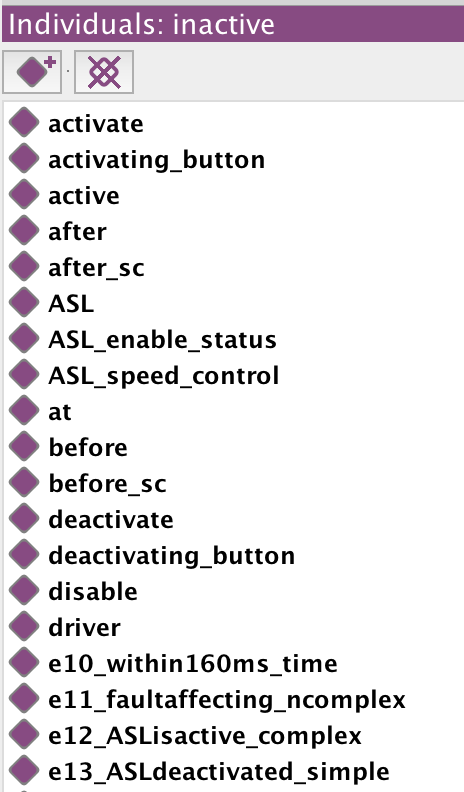
\includegraphics[width=0.3\textwidth]{images/ro_individuals} 
} 
	\caption{Requirements specification ontology (screenshot from Prot\'eg\'e tool).} \label{fig_ontology}
\end{figure}

In order to strengthen the analysis, lexical relations between arguments are introduced such as antonyms, synonyms, generalization, specialization, e.g., the fact that ``enabled'' is antonym of ``disabled'', generalization of components by their container (or system), e.g., the relationship between ASL and its components, etc. Once the ontology is constructed considering the event-based semantic, thematic roles, lexical relation, we check the consistency of it via an inference engine (or reasoner), which is a software program that applies logical rules on a logical system, such as the ontology, to obtain new information.
\begin{definition}
 The ontology is consistent if there exists an interpretation (or a model) $M$ that satisfies the terminological assertions $T$ and the concrete assertions $A$, that is, $M \models ax$, where: $ax \in T \cup A$, where $T$ is a set of terminological assertions, such as InParameter $\subset$ Parameter, and A is a set of facts (or concrete assertions).
\end{definition}

\section{Formal and Scalable Analysis of Simulink Models}\label{rc_sim}
A Simulink model consists of functional blocks, which are modeling elements to realize some functionality, e.g., generate signal, delay a signal, mathematical operations over signals, etc., and lines connecting the blocks. The Simulink block can be either discrete or continuous depending on the block's execution behavior. If the block is executed periodically with a sample time $t_s$, it is discrete, otherwise, it is continuous if it has no sampling time, rather executes over finitely small (or minor) sampling times. The blocks can also be classified into atomic and composite blocks, where the atomic blocks, e.g., a delay block, is atomic schedulable entity that cannot be decomposed further. Whereas, the composite blocks, e.g., the Subsystem block, contains atomic blocks, and is used to create hierarchy, hence improving the visualization or to impose collective execution behavior over a set of atomic blocks. 

\subsection{Semantics of Simulink Model in Network of STA} 
The semantics of a Simulink model is given as a network of stochastic timed automata, which is defined as a composition of independently executing automata (processes). The automata are labeled transition systems which denote the semantics of Simulink blocks, and the syntax of a block is captured as a tuple 

\begin{definition}[Simulink model]
	\label{def:Simmodel}
	A Simulink model is formally defined as a sequential composition of n Simulink blocks that communicate via shared variables, as follows:
	\begin{equation}\label{blocksyntax}
	S = B_1 \otimes B_2 \otimes B_3 \dots \otimes B_n,
	\end{equation}
\end{definition}  
where: $ B_1, B_2, \dots, B_n $ are computational Simulink blocks and $\otimes$ is a  composition operator. 

The syntax of a Simulink block is given as a tuple $\langle s_n, V_{in}, V_{out}, V_{D}, \Delta, Init, blockRoutine \rangle$, where $s_n$ is the execution order of the block, $V_{in},V_{out}$ and $V_{D}$ are the set of input, output and state variables of the block. $\Delta$ are the set of sample hits, when block update functions are executed. The $Init$ and $blockRoutine$ functions performs initialization of the block's state variables and executes the update functions of the block, respectively.
\begin{definition}[Semantics of a Simulink block] 
	\label{def:semantics-Simblock}
	Assume $B$ is a Simulink block, the semantics of $B$ is a timed transition system
	$T_B = \langle q_0, Q, \mathcal{L}, \longrightarrow \rangle$, where 
	\begin{itemize}
		\item $Q$ = $\mathbb{R}^n$ is the state space given by the values of all output variables $y$ at a given time instance $t \in \mathbb{R}_{\geq 0}$, for given input at time $t$
		\item  $q_0 = y_0|_{t_0} = (y_0, t_0) \in Q$ is the initial state at $t_0\in \mathbb{R}_{\geq 0}$
		\item $\mathcal{L}$ = $\mathcal{L}_a \cup \mathcal{L}_t$ is the set of labels, with $\mathcal{L}_a$ the set of action labels $\{Init, blockRoutine\}$, and  $\mathcal{L}_t$ the set of time labels $\{r* \delta, m*\delta\}$
		\item $\longrightarrow$ is the transition relation from $\longrightarrow \subseteq Q \times \mathcal{L}_a \times \mathcal{L}_t \times Q$,
	\end{itemize}
\end{definition}% 
where $r*\delta\in \mathbb{R}_{\geq 0}$ are the set of sample hits that occur every infinitesimal sample time $r$, to approximately model the continuous behavior of blocks, and $m*\delta$ are the sample hits that occur every sample time $m$, to model the behavior of discrete blocks. We refer the reader to Section~3 of our paper \cite{Filipovikj2018SimppaalModels} for the detailed formalization discussion.

\noindent\\ \textbf{Transformation Patterns: } In order to facilitate the transformation of the Simulink blocks into their equivalent transition systems, we propose two types of transformation patters for the continuous-time and discrete-time blocks. The transformation patterns are reusable and they conform to the semantics of the tuple introduced in Equation~\ref{blocksyntax}. Figure~\ref{fig_patterns} shows our transformation patterns encoded in the input language of \uppaalsmc.
\begin{figure}[] 
	\centering
	\subfloat[Continuous.\label{fig_continuous}]{% 
		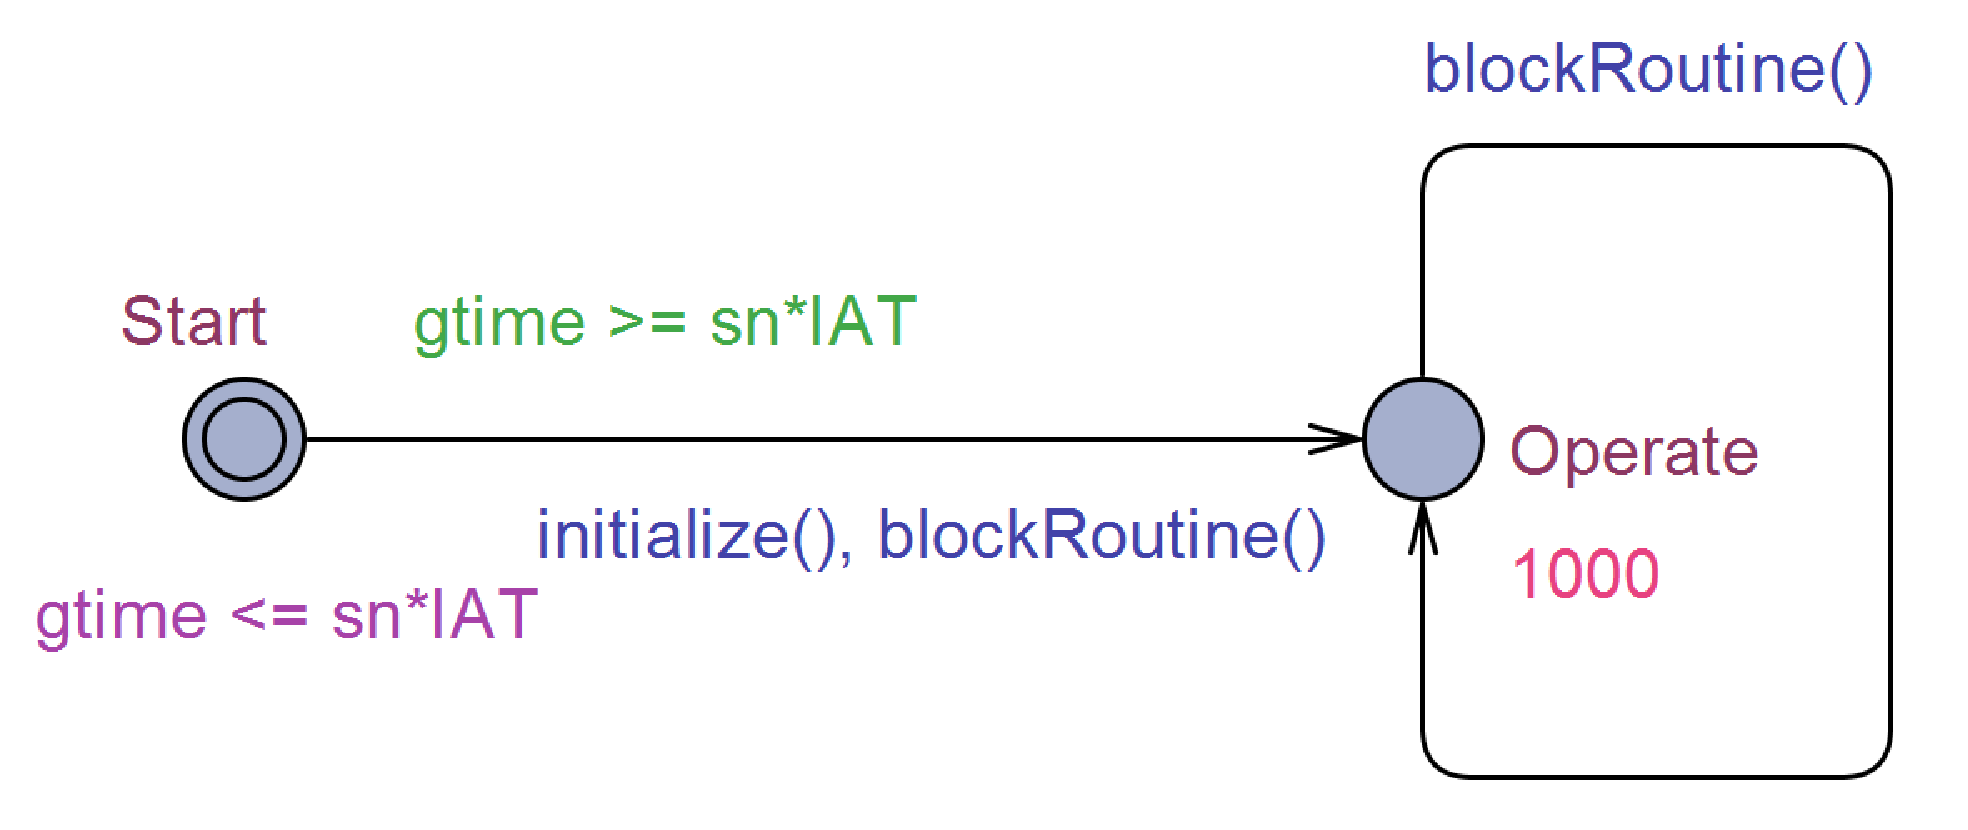
\includegraphics[width=0.5\textwidth]{images/continuous.pdf}
	} ~
	\subfloat[Discrete.\label{fig_discrete}]{% 
		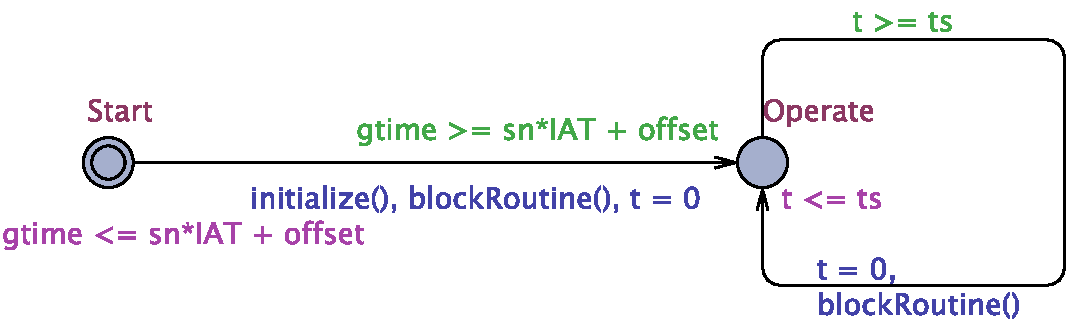
\includegraphics[width=0.5\textwidth]{images/discrete.pdf}
	} 
	\caption{STA transformation patterns.} 
	\label{fig_patterns}
\end{figure}

Each pattern has its own execution mechanism. The execution of continuous-time patterns presented in Figure~\ref{fig_continuous} proceeds according to an exponential distribution for unbounded delays, whereas the execution of the discrete-time pattern presented in Figure~\ref{fig_discrete} proceeds according to the uniform distribution for time-bounded delays modeled via the invariant.

To check the correctness of the \texttt{blockRoutine} functions, which we implement in the subset of the C language used by \uppaalsmc{}, we use pre-/post-condition verification using the Dafny program verifier. A set of pre-conditions is used to describe the input, output and state variables prior to the execution of the \texttt{blockRoutine}. Given that the pre-condition holds, after the execution of the blockRoutine, the set of post-conditions has to be established. We consider the \texttt{blockRoutine} to be correct if the specified set of postconditions is satisfied for all executions. For complex block routines that contain loops, we use loop invariants and termination conditions. The detailed description of the verification procedure for the \texttt{blockRoutine} using \texttt{Dafny} has been omitted for brevity. 

\noindent\\ \textbf{Transformation process:} The network of automata is automatically generated from the Simulink model by applying the following steps, as also illustrated in Figure~\ref{fig_approachworkflow}:
\begin{description}
	\item[Step 1] The Simulink model is simulated, subsequently, the sorted-order list, which contains the execution order of the Simulink blocks, is extracted.
	\item[Step 2] In case the model is hierarchical, the execution order is flattened first, thus generating a flattened sorted-order list.
	\item[Step 3] The Simulink model is parsed, as a result, each block is translated into a stochastic timed automata via a transformation pattern, which takes its block routine and the flattened sorted-order list.
	\item[Step 4] In the transformation, the continous-time STA and the discrete-time STA patterns are applied to continuous-time and discrete-time blocks, respectively.
	\item[Step 4] the connections between blocks are translated into input-out variables of the automata 
\end{description}

\begin{figure}
	\centering
	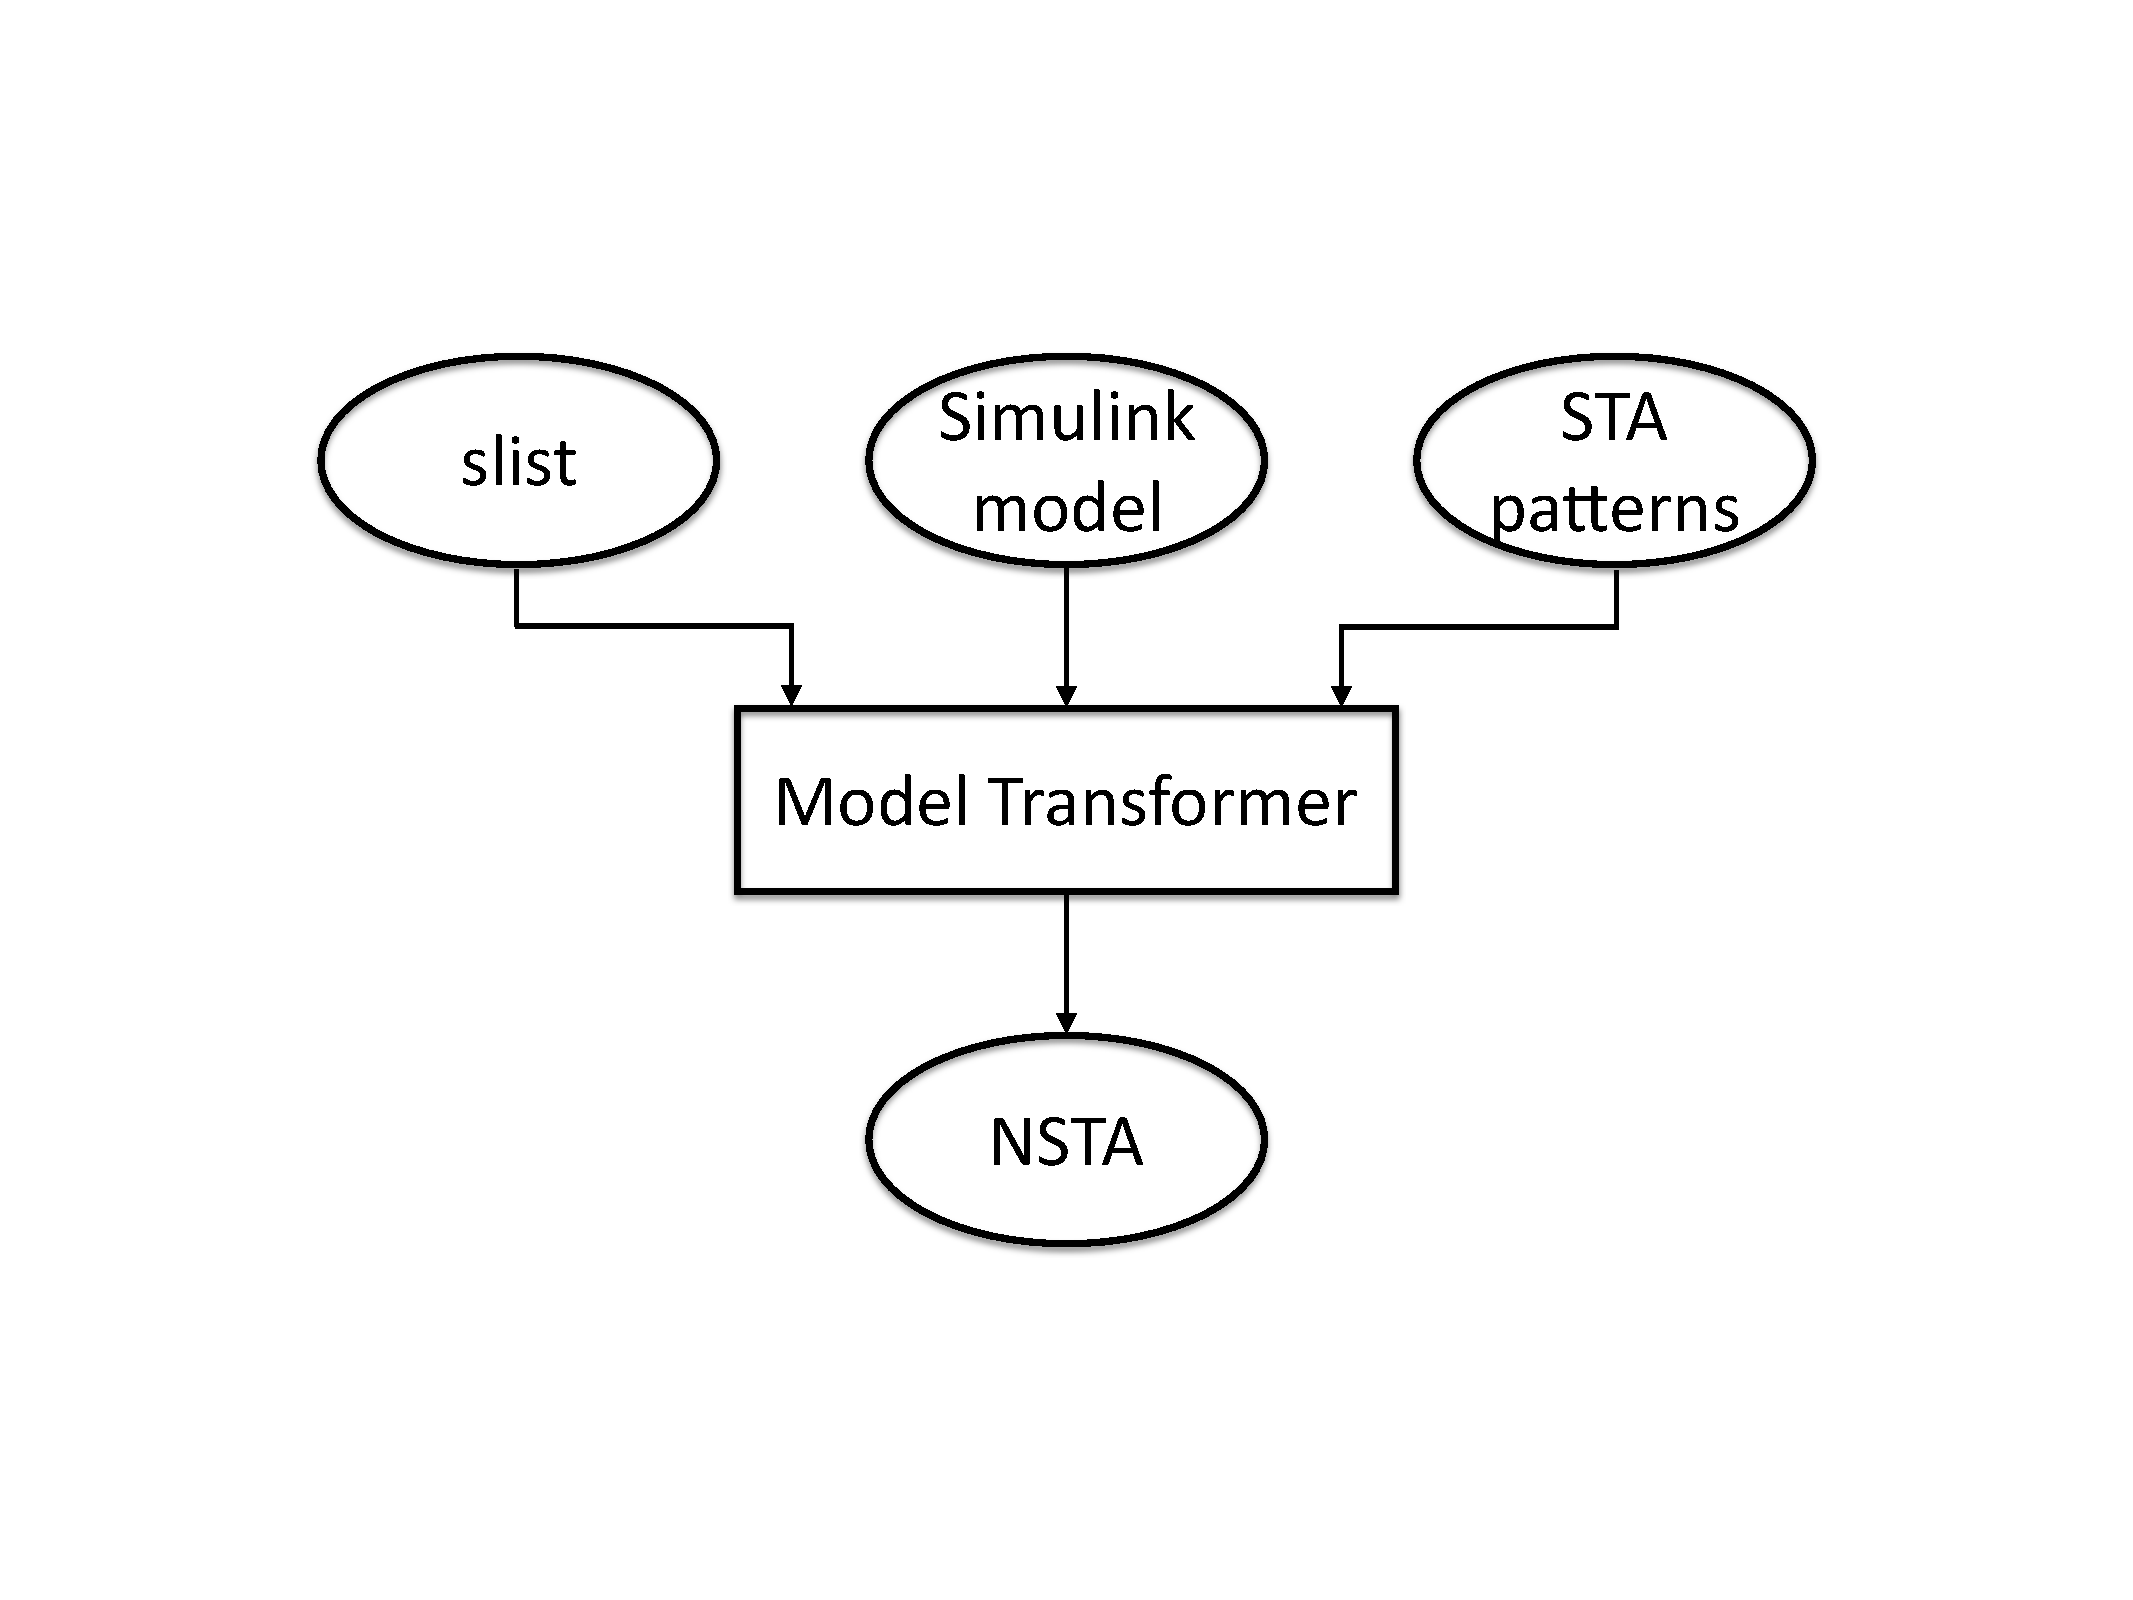
\includegraphics[width=0.6\linewidth]{images/simulinkapproach}
	\caption{Simulink to NSTA Transformation}
	\label{fig_approachworkflow}
\end{figure}

\subsection{Validation on the Brake-by-wire System} 
To validate the proposed approach, we use a brake-by-wire use case that is obtained from Volvo Group Trucks Technology. The brake-by-wire system controls the vehicle speed using sensors and actuators, e.g., by reading the pedal position, vehicle speed, etc., and employs an elctromecahnical control system to compute the proportional torque force that is applied on the wheels. Besides realizing the braking functionality, the model realizes anti-braking functionality to avoid (or minimize) skidding, which occurs when the slip rate of a wheel is greater than its friction coefficient.  The anti-braking feature is activated whenever the vehicle speed is greater than 10km/hr.

The brake-by-wire Simulink model contains 320 blocks which is structured into a 4-level hierarchy, and consists of continuous and discrete blocks. Following the transformation, the model is first simulated in Simulink, subsequently, the sorted-order lists is extracted. Then, the model is transformed into a netwok of stochastic timed automata via the transformation patterns. Note: the timing behavior of the automata complies to the sorted order list, thus preserving the exectuiong semantics of the Simulink model.

\section{Exact Software Allocation  via ILP}\label{rc_ilp}
Safety-critical systems are usually resource constrained, that is, the execution hardware platform has limited computational resources and power/energy sources. Therefore, the system should be designed efficiently especially critical system resources such as power in order to accommodate complex safety-critical software functionality. In this section, we propose exact method of mapping software to hardware in order to optimize the total power consumption of a distributed safety-critical software via ILP, which is needed when highly-efficient design is needed especially small-scale sofware applications, e.g., software components not exceeding 10.

We consider an AUTOSAR distributed safety-critical software that can be mapped to multiple computing nodes (or units), which are heterogeneous computing systems with respect to power specification, failure rate and processing speed. The software has end-to-end timing and reliability requirements, therefore, the mapping must satisfy the requirements. In order to meet the reliability requirement, the mapping applies fault tolerance by replicating software components subsequently mapping the replicas on different computing units. Moreover, the task and messages that realize the safety-critical software functionality are scheduled using a fixed-priority preemptive scheduling policy and fixed-priority non-preemptive scheduling policy (over a  CAN bus), respectively.

The AUTOSAR software functionality is implemented by Runnables that communicate over the virtual function bus (VFB), which abstracts the details of the run-time environment. We assume the runnables are triggered periodically and have multiple worst-case execution times as they can executed on processors that have different processing speed.

\subsection{ILP Model Formulation}
Consider that the mapping solution is represented by a vector of binary matrices $\textbf{x}=\{\textbf{x}_1:1,...,K\}$, where \ttxkij represents the mapping of the software component $\sss{q}[k][ij]$ to the computing node $\ssb{n}[j]\in \mathcal{N}$. 
\begin{equation}
\label{eqn_solution}
\bspx{k}=
\begin{bmatrix} 
\ssx{k}{11} & \ssx{k}{12} & \dots & \ssx{k}{1K}\\
\ssx{k}{21} & \ssx{k}{22} & \dots & \ssx{k}{2K}\\
\vdots & \vdots & \ddots & \vdots\\
\ssx{k}{N1} & \ssx{k}{N2} & \cdots & \ssx{k}{NK}
\end{bmatrix}
\end{equation}
The power consumption of a software application $\{c_i:i=1,...,n_C\}$ that is mapped to computing units $N'\in N$ is calculated as the sum of the power consumption of each node $n_h\in N'$, thus $\mathcal{P}_{total}(x)=\sum_{n\in N'}{\mathcal{P}(u_n(x))}$, where $\mathcal{P}(u)$ is the power consumption of a computing node which linearly proportional to its utilization~\cite{Mahmud5222}. The utilization of a computing node is the sum of the utilization of its constituent tasks that realize corresponding software components.
\begin{align}
	(u_1,...,u_K)(\x)=\sum_{k=1}^{K}\sum_{\tau\in T_{c_i}}{\xkij*\frac{WCET_\tau}{P_\tau}},
\end{align}
where $T_{c_i}$ is the set of tasks realizing the software component $c_i$, $WCET_\tau$ and $P_\tau$ are the worst-case execution time and  period of the task $\tau$.

\subsubsection{Tasks Deadline Constraint}
The mapping solution must satisfy the timing and reliability requirements imposed on the safety-critiacal application. We assume the taskset in each computing node is scheduled using a fixed-priority preemptive scheduler~\cite{Sha2004RealPerspective} and we check the schedulability via the classical worst-case response time analysis~\cite{Baruah2011Response-timeSystems}. Since the time analysis model involves recursion which is difficult to model as a linear model. Therefore, we construct linear logical constraints $\xi$ that corresponds to the valid tasksets that can potentially partitioned to computing nodes, and these tasksets are schedulable.

The logical system is constructed as follows: first we identify the possible partitions of the software components, $P=2^C$, then we check the schedulability of each partition and catagorize them per node, i.e., $Y_j=\{p\in P| isSched(p,n_j)\}$, where $sched$ is a boolean function that returns true if $p$ is schedulable on $n_j$.  A partition is identified by a sequence of 0s and 1s based on its costituent components, e.g., the id of the partition $\{c_1,c_4,c_5\}\subseteq \{c_1,c_2,c_3,c_4,c_5\}$ is $10011=19$. So, given the mapping $\x$, the partition id that is mapped to the computing node $n_j$ can be computed as
\begin{align}
	g_j(\x)=\sum_{i=1}^{N}{10^{N-i}\max_{1\leq k< K}\xkij}
\end{align}
where the $\max_{1\leq k< K}$ function returns 1 if at least one component replica is mapped $n_j$, otherwise returns 0, indicating no replica is mapped to that node. Thus, each node must have a valid partition that is schedulable as indicated in the logical constraint,
\begin{align}
\bigvee\limits_{p\in Y_j}g_j (\x)= id(p) ,
\end{align}
where $id(p)$ is a predicate that returns the id of the partition $p$.

\subsubsection{End-to-end Timing Constraint}
The age delay of a chain is computed according to the semantics discussed in~\cite{Feiertag2009ASemantics}\cite{mubeen2013support}. The response-time logical assertions ensure that every task in the distributed system are schedulable for a mapping \ttx. Therefore, we can safely check if the age delay of each chain satisfy its end-to-end timing requirement without the need to check the chain's constituent tasks are schedulable or not. Similar to the previous approach, we construct logical constraints $\eta$ that correspond to the valid set of mappings of chains on the network of computing nodes.  Given $\Gamma =\{\Gamma_i:i=1,...,N\}$ of chains, the set of possible mappings of each chain $\Gamma_i$ on a set of $\mathcal{N}^\Gamma$. Thus the set of valid mappings of each chain satisfy the end-to-end timing requirement is $Z_i=\{\gamma\in \mathcal{N}^\Gamma| ageDelay(\gamma) < EE_\gamma$.

\subsubsection{Software Application Reliability Constraint}
The reliability constraint refers to the probability that the application functions by the time $t$, i.e $[0,t]$~\cite{Goel1985SoftwareApplicability}. We assume that the reliability requirement of a software application is 0.99999999 over a 2-year operation time, which is to say  that the safety-critical system almost should not fail within the stated period. Furthermore, we assume that the mean-time to failure of the computing nodes is given as $10^6$ hours (0.0000001 per hour), which is the usual practice in many functional safety design.

Unless the the software application is replicated on one or more computing nodes, the reliability requirement is usually unattainable. So, the allocation strategy is basically to replicate sufficient software components to meet the requirement at the same time it should not exceed the limit so that the application consumes less power. However, the reliability calculation is not trivial as the replication results in functional inter-dependency of the computing nodes, in this case,  the series-parallel method does not apply. For this reason, we propose an exact method based on state enumeration~\cite{ExactMethodstoComputeNetworkRe- liability}, which basically enumerates all the possible configurations of the nodes  $PS$. Subsequently, the reliability of the application becomes the total probability of the configurations that enable the functioning of the application~\cite{Mahmud5222}.
\begin{definition}[Software Application Failure]
	A software application fails in the configuration $s\in\xi$ if there exists a component type $c_i$ where all of its replicas $Q_i$ \textit{fail}, otherwise, it functions, as shown in Equation (\ref{eqn_appreliability_milp_components}).  The component replica $q_i,j\in Q_i$ of type $c_i$ fails if $n_h$ fails, that is $s_h=0$.
\end{definition}
\begin{align}
f_s(x) = \floor[\Bigg]{\frac{\sum_if_{c_i}(x,s)}{N}}=
\begin{cases}
1 & \mbox{if } application \mbox{ functions}\\
0 & \mbox{if } application \mbox{ fails}
\end{cases}\label{eqn_appreliability_milp_components}
\end{align}

Thus, the reliability of the software allocation is
\begin{align}
\label{eqn_appreliability_milp}
Reliability(\x)=\sum_{s\in PS}f_s(\x)*p_s,
\end{align}
where $p_s$ is the probability that the computing nodes attain a configuration $s$ which is computed as $p_s=\prod_{m\in M}\big[(z_m*\lambda_m) + (1-z_m)*(1-\lambda_m)\big]$, where $z_m\in\{0,1\}$ indicates if the node fails (i.e., 0) or functions (i.e., 1), $\lambda_m$ is the failure rate of the node $m$ and $1-\lambda_m$ is the opposite of failure rate, i.e., that is the rate that it does not fail.
\subsubsection{ILP Problem}
The goal of the ILP optimization is to minimize the total power consumption, which is the objective function, and the constraints Equation (\ref{lbl_deadline_constraint}), (\ref{lbl_e2e_constraint}) and (\ref{lbl_reliability_constraint})ensure that the optimization satisfies the tasks deadline, end-to-end timing and reliability constraints, respectively.
\begin{align}
\label{eqn_const_func}
\min_{\x\in X} \mathcal{P}_{total}(\x) && \text{ Subjected to:}\\
\label{lbl_deadline_constraint} 
\bigvee\limits_{p\in Y_j} g_j (\x) &= id(p)& \mbox{ for all } j=1,..,|\mathcal{N}|\\ 
\label{lbl_e2e_constraint}
\bigvee\limits_{\gamma\in Z_j} h_j (\x) &= id(\gamma) & \mbox{ for all } j=1,..,|\Gamma|\\ 
\label{lbl_reliability_constraint}
\sum_{s\in PS}f_s(\x)*p_s &\leq \RL&,
\end{align}

\subsection{Tool Support and Validation on Automotive Benchmark}
Our proposed ILP approach is validated on different size of software applications, i.e., applications with variable number of software components, cause-effect chains and degree of replication. The applications are synthesized according to the automotive benchmark proposed by Kramer et al.~\cite{Kramer2015RealFree}, which discusses a typical complexity of an AUTOSAR engine management system in terms of, e.g., the number and execution time of runnables, and the number and activation patterns of cause-effect chains. 

We prepared 6 software applications and an execution platform that consists 8 nodes. The smallest application consist of 4 components and the largest 10 components. Furthermore, the cause-effect chains varies from 10 to 60 and activation patters ranges from 2 to 4. Figure~\ref{fig_ilp_results} shows the result of the optimization from the CPLEX solver, that is, the power consumption and the computation time, respectively. In general, the optimization maps components to nodes with lower power specification and higher processor speed, however, this is not always the case since the end-to-end timing and reliability constraints can dictate the selection of different nodes, which consume more power as a result. Figure~\ref{fig_computationtime_ilp} shows a slow increase of computation time from until the application with 8 number of components, which took  6.06 sec, and rapidly increased to 30.3 sec and 129.4 sec allocating application with 9 and 10 components, respectively. The optimization took extremely large amount of time for applications that consist of more than 10 components, and more than 15 component the waiting time was intractable, thus the optimization was interrupted manually. 
\begin{figure}[h] 
	\centering
	\subfloat[Power consumption of nodes.\label{fig_powerconsumption_ilp}]{% 
		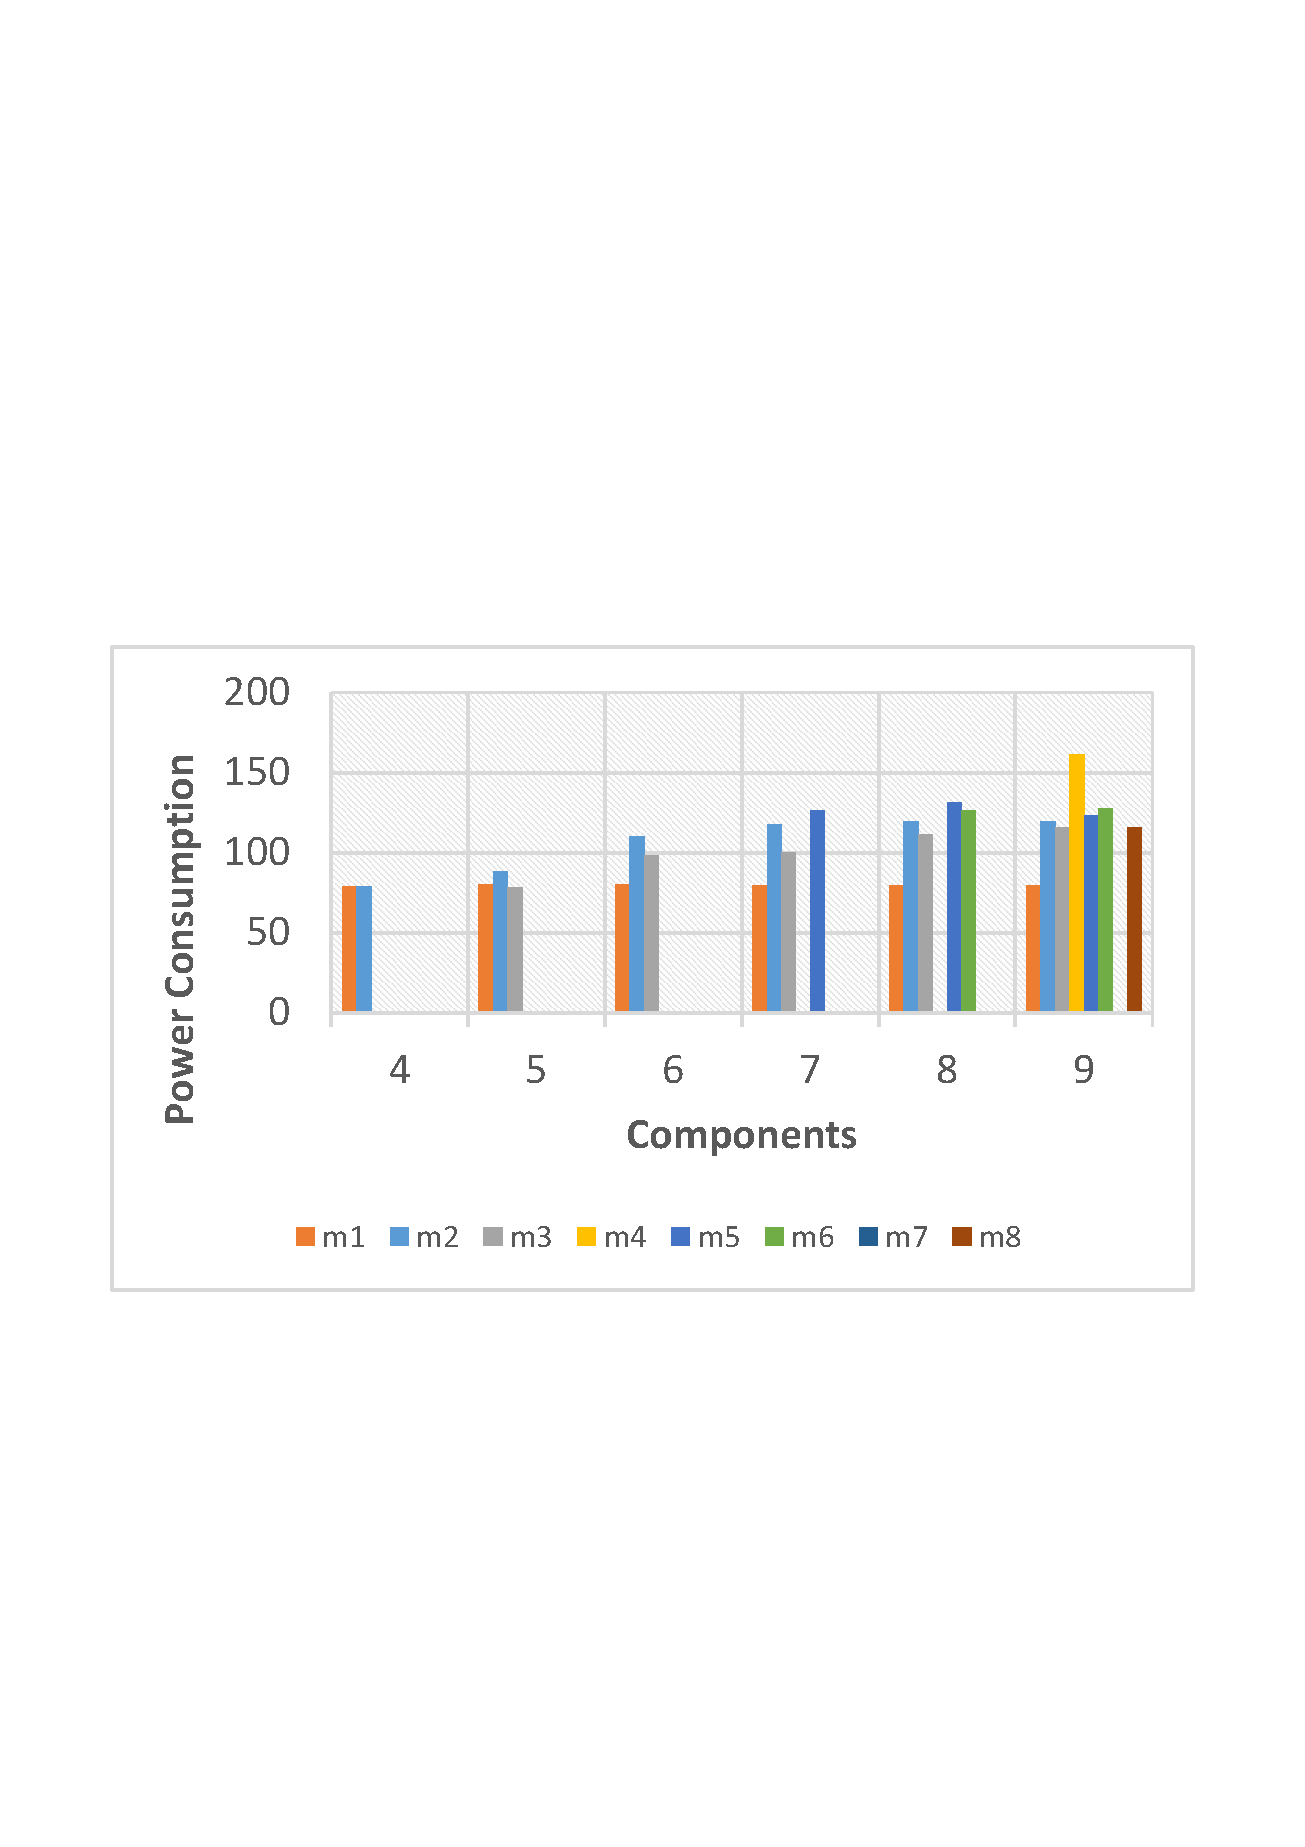
\includegraphics[width=0.45\textwidth]{images/power}
	} ~
	\subfloat[Allocation times software applications.\label{fig_computationtime_ilp}]{% 
		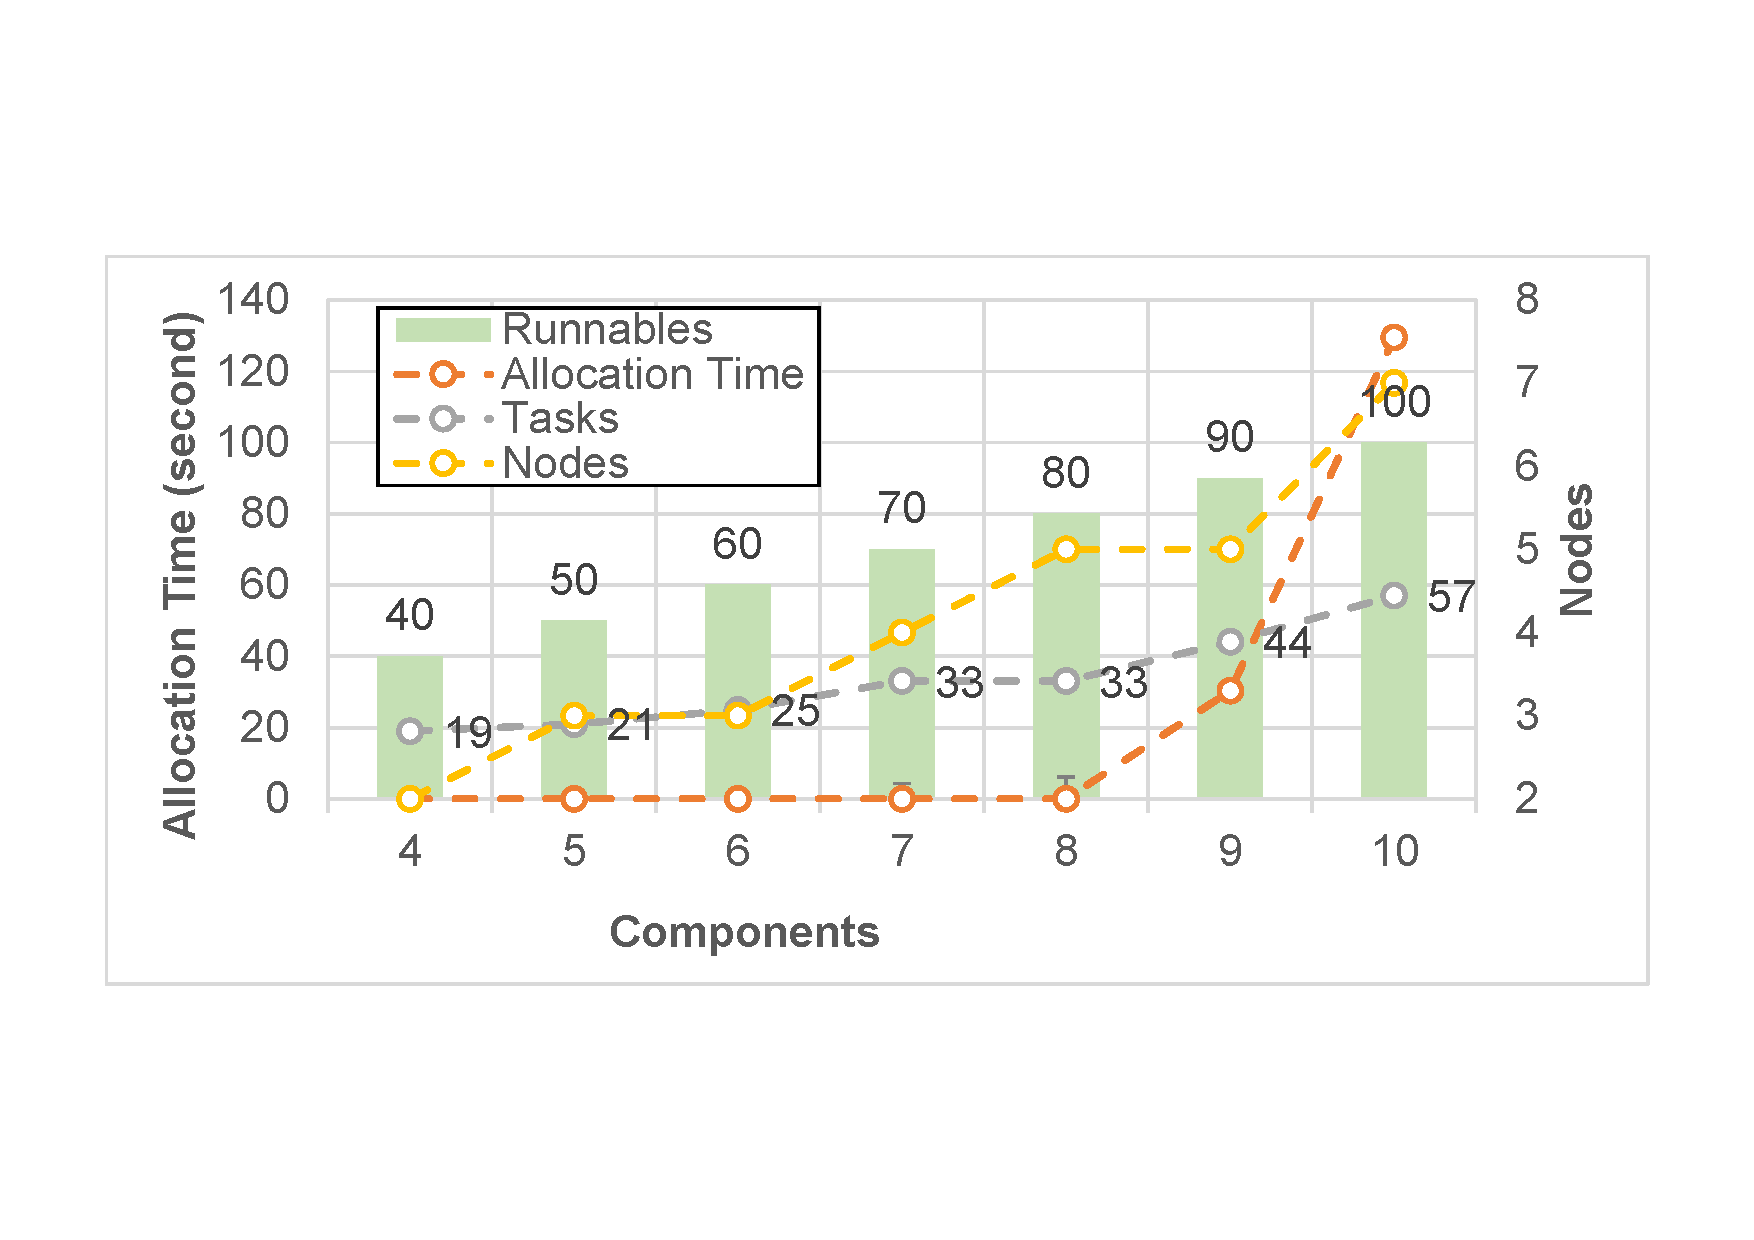
\includegraphics[width=0.55\textwidth]{images/increasing_components} 
	} 
	\caption{ILP optimization of different sizes of software applications based on the number of software components, cause-effect chains, computing nodes.} \label{fig_ilp_results}
\end{figure}

\section{Scalable Software Allocation via Hybrid PSO}\label{rc_pso}
In the previous contribution, we observe that the ILP approach does not scale well to the large software allocation problems. To address this problem, in this section, we propose approximation algorithms based on metahuristics, which is ``high-level problem-independent algorithmic framework that provides a set of guidelines or strategies to develop heuristic optimization algorithms''. Meta-heuristic algorithms does not guarantee optimality of solutions, nevertheless, the solutions can be deemed satisfactory. In the case of minimizing power consumption, what is more appealing to system designers is usually the benefit attained as a result of the power consumption reduction, e.g., accommodating more and more software applications, improving battery-life, rather than optimality. In this spirit, metahuristics can be useful to solve complex and large optimization problems, yet in reasonable time, as compared to exact methods, e.g., branch-and-bound, dynamic programming.

\subsection{Hybrid Particle-swarm Optimization}
The canonical \pso{} technique uses the constriction factors to balance exploitation and exploration of the search space to get closer to the global optima, hence improving solution quality. Nevertheless, it still suffers from premature convergence or local minima especially when applied on complex and large problems~\cite{Rini2011ParticleChallenges}. Its hybridization is proven to perform better in many cases~\cite{Sengupta2018ParticlePerspectives}. In particular, it is shown to perform better in the tasks assignment problem, that is when hybridized with, e.g., the genetic algorithm~\cite{Sailer2013OptimizingAUTOSAR}, the hill-climbing~\cite{yin2007task}, simulated annealing~\cite{Zhao2007ASystem}, differential evolution~\cite{Storn1997DifferentialSpaces}. As compared to the hybridization with genetic, the hybridization with hill-climbing \hcpso{} is shown to perform better by Yin et al.~\cite{yin2007task} for the tasks allocation problem to maximize reliability of distributed systems. 

In this work, we apply \hcpso{} to the problem at hand, and to tackle its stagnation when applied to large problems. Moreover, we hybridize \pso{} with the differential evolution technique, \depso{}, to improve diversification by applying the mutation and cross-over operators of the differential evolution. Algorithm~\ref{alg_depso} show the pseudocode of the hybrid \pso{}. Line 3 and 4 compute the personal best and the swarm best solutions, respectively. For each particle in the swarm, the velocity and position is computed in Lines~5-8. Lines~9-13 apply the hybridization based on the choice of the algorithm, i.e., \de, \hcpso{} and \shpso{} intermittently, i.e., whenever the interval criterion condition is met.
\IncMargin{1em}
\begin{algorithm}[H]
	\SetAlgoLined
	\SetKwData{P}{P}\SetKwData{S}{sBest}
	\SetKwData{Generation}{Generation}
	\SetKwData{Interval}{Interval}
	\SetKwData{Particles}{Particles}
	\SetKwInOut{Input}{input}\SetKwInOut{Output}{output}
	\SetKwFunction{OptimizeUsingDE}{optimizeUsingDE}
	\SetKwFunction{OptimizeUsingHC}{optimizeUsingHC}
	\SetKwFunction{OptimizeUsingSHC}{optimizeUsingSHC}
	\SetKwFunction{ComputeParticleVelocity}{computeParticleVelocity}
	\SetKwFunction{ComputeParticlePosition}{computeParticlePosition}
	\SetKwFunction{InitPSO}{initPSO}
	\SetKwFunction{ComputePersonalBest}{ComputePersonalBest}
	\SetKwFunction{ComputeSwarmBest}{ComputeSwarmBest}
	
	\BlankLine
	\Input{\pso parameters, \de parameters}
	\Output{Software allocation solution \S .\textbf{x}}
	\BlankLine
	\Particles $P$ $\leftarrow$ \InitPSO{}\;
	\BlankLine
	\While{termination criteria}{
		$\textbf{p}_{bst}$ $\leftarrow$\ComputePersonalBest{$P$}\;
		$\textbf{z}\leftarrow$\ComputeSwarmBest{$P$}\;
		\BlankLine
		\ForEach{$p\in P$}{
			\ComputeParticleVelocity{$p$} according to Equation (\ref{eqn_pso_velocity})\;
			\ComputeParticlePosition{$p$} according to Equation (\ref{eqn_pso_position})\;
		}
		\If{interval criteria}{
			$P$ $\leftarrow$ \OptimizeUsingDE{$P$}\;
			\tcp{$P$ $\leftarrow$ \OptimizeUsingHC{$P$}}\label{hc}
			\tcp{$P$ $\leftarrow$ \OptimizeUsingSHC{$P$}}\label{sh}
		}
	}
	\caption{Hybrid \pso{} Pseudocode.}
	\label{alg_depso}
\end{algorithm}\DecMargin{1em}

\subsection{Validation on the Bosch EMS Benchmark} 
In this section, we evaluate our proposed hybrid \pso{} algorithms for the allocation of software applications to heterogeneous computing units. The algorithms are evaluated against different specifications of automotive software applications and execution platforms with regard to effectiveness, stability and scalability. The software-application specifications consist of the number of software components $c$, runnables $r$, tasks $t$ and cause-effect chains $g$.  The specifications are synthesized from the automotive benchmark proposed by Kramel et al.~\cite{Kramer2015RealFree}. The benchmark indicates a strong correlation between runnables and cause-effect chains in terms of timing and activation patterns. It shows the timing specifications of runnables and their shares in an engine management system. Moreover, it shows the activation patterns of cause-effect chains, the runnables per activation and their shares in the system. The engine management system is one of the most complex automotive systems in the vehicular electrical/electronic execution platform. 

\noindent\\ \textbf{Result:} We conducted two experiments: i) the first experiment is designed to compare the performance such as the convergence time, computation time, optimality (or quality of solutions) and stability of the meta-heuristic algorithms used in this paper, ii) the second experiment is designed to evaluate the overhead of increasing replication on the optimization especially due to the computation of end-to-end delays, and also to evaluate the effect of the approximation algorithm proposed to reduce the overhead.

In the first experiment, as illustrated in Figure~\ref{fig_powerconsumption_ilp_metaheuristic}, we show that \ilp returned optimal solutions in the first three problems, likewise all except \pso{} and \depso{}. However, as the problem size increases, the computation time became exponential as shown in Figure~\ref{fig_allocationtime_ilp_metaheuristic} and did not return solutions. In contrast, the hill-climbing-\pso{} hybrid performed the best in all last three problems except \hcpso{} failed to return near optimal solutions to the largest problem \pb{80}{20}{60}. The result also shows that the stochastic version of the hill-climbing-PSO hybrid \shpso{} scales better the over quality of the solution can deemed acceptable as compared to the \ilp{} in the first three problems and \hcpso{} in the next two problems. 
\begin{figure}
	\centering
	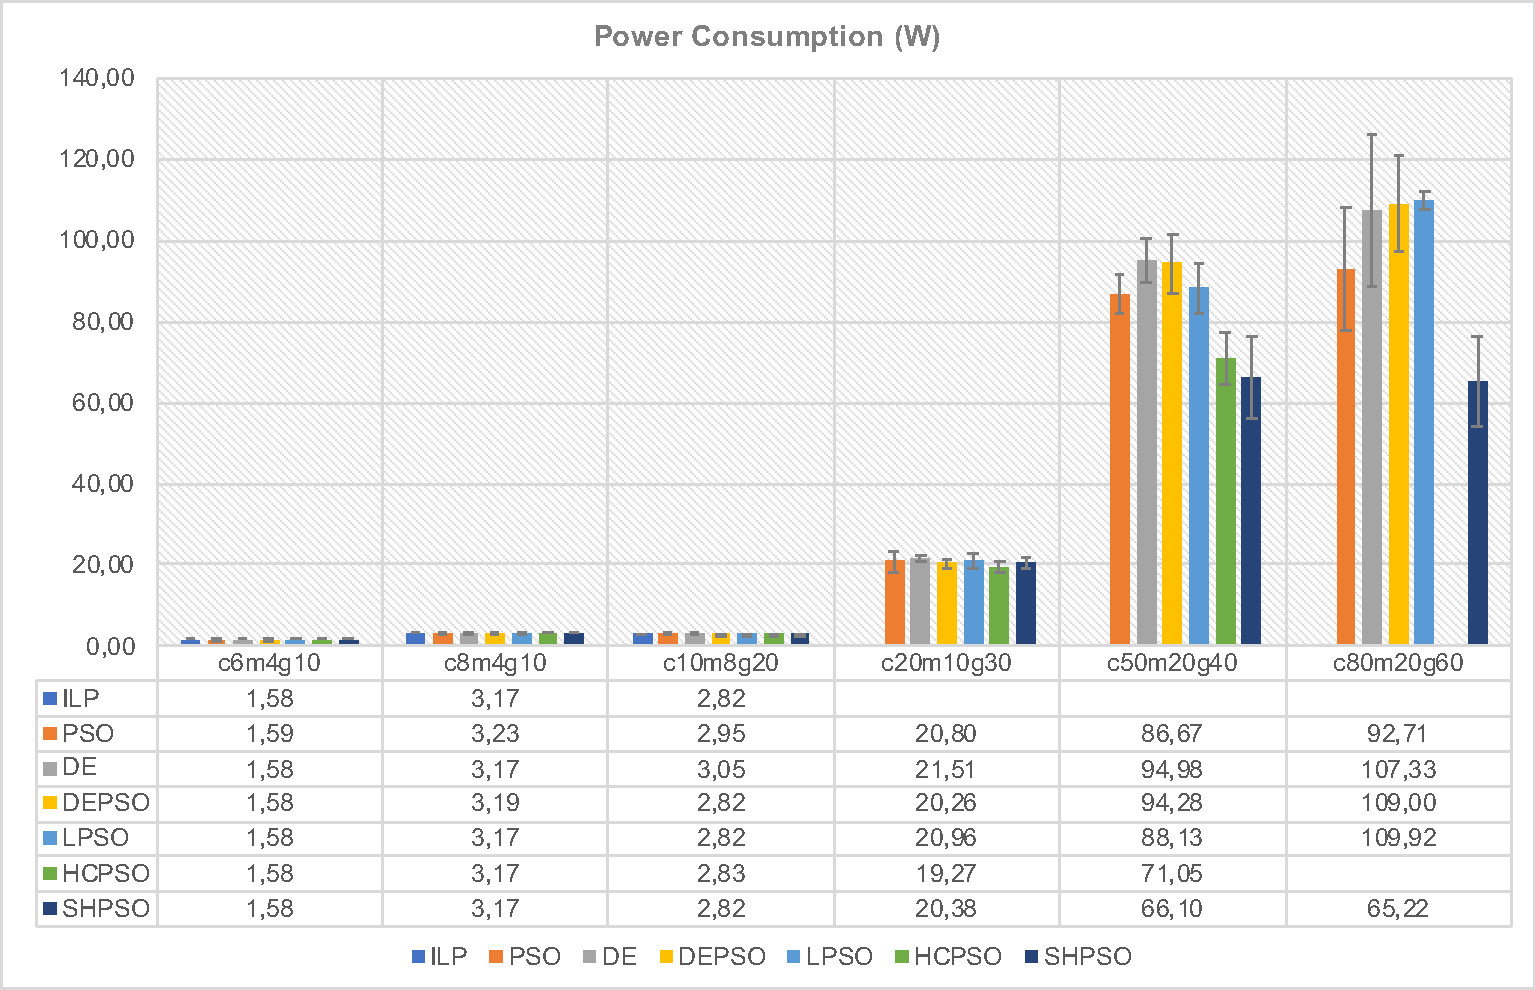
\includegraphics[width=0.8\linewidth]{images/power_consumption.pdf}
	\caption{(Near) Optimal Power Consumption of the Different Software Allocation Problems.}
	\label{fig_powerconsumption_ilp_metaheuristic}\vspace{-0.4cm}
\end{figure}

\begin{figure}
	\centering
	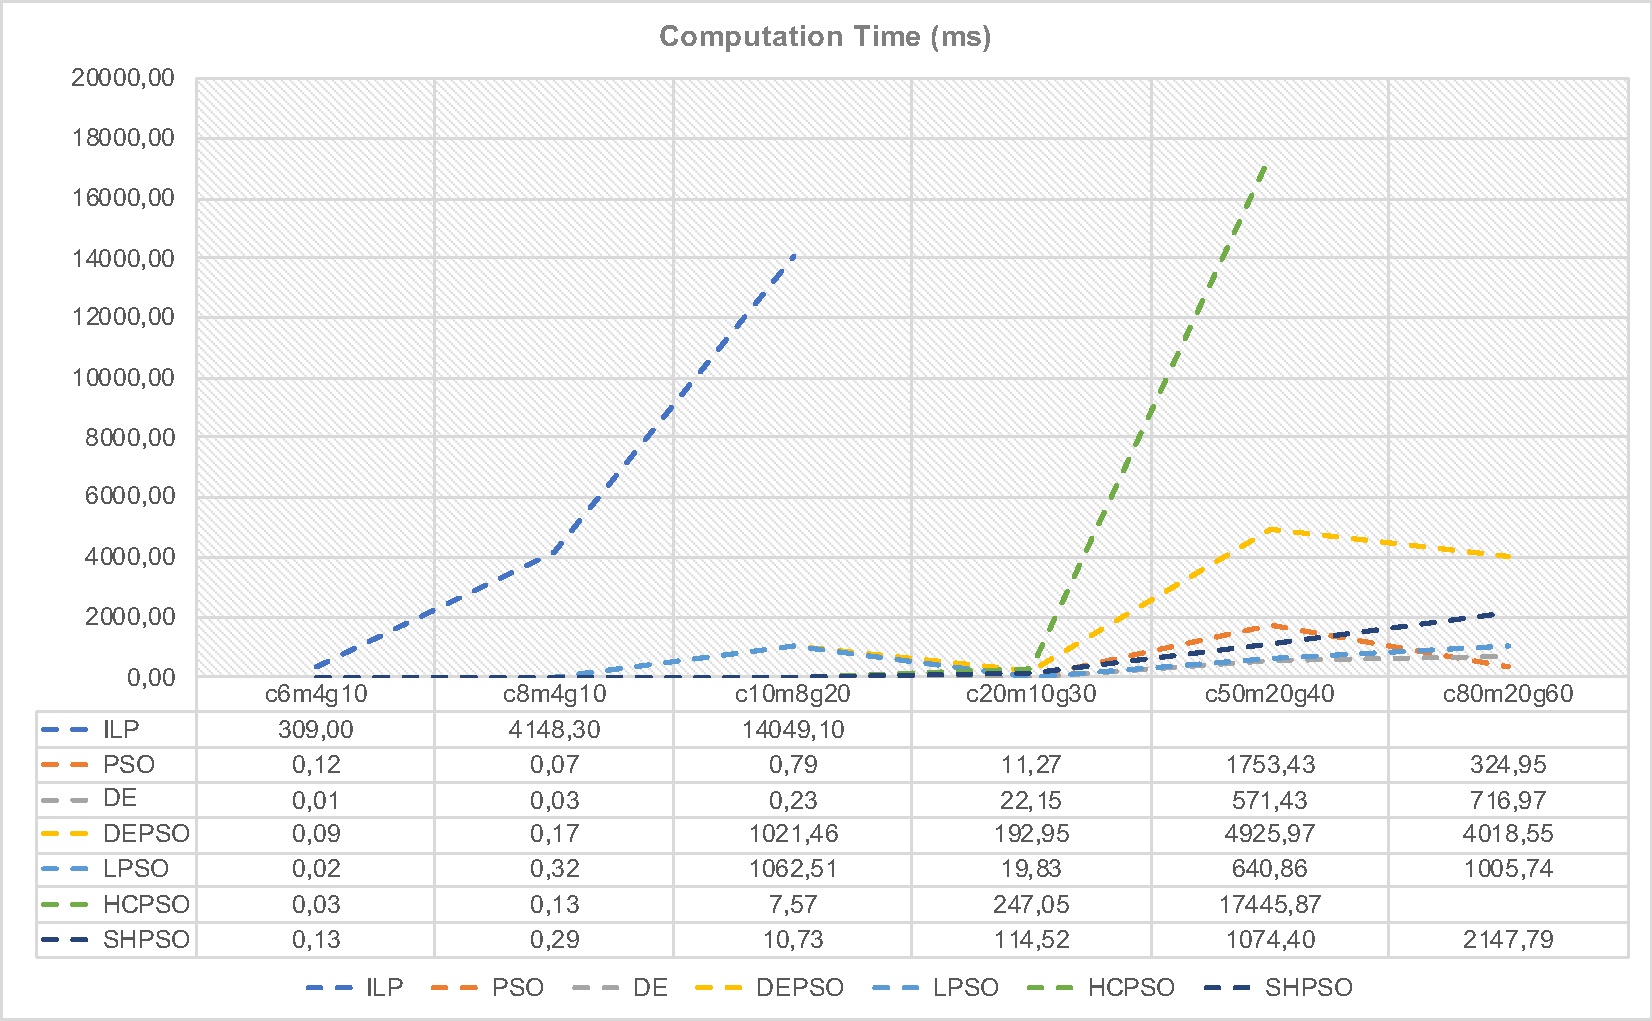
\includegraphics[width=0.8\linewidth]{images/time_summary.pdf}
	\caption{Computation time of the various algorithms for solving different instances of the software allocation problem.}
	\label{fig_allocationtime_ilp_metaheuristic}\vspace{-0.4cm}
\end{figure}

Due to the replication of software components to the reliability goals of the software applications, the overhead of computing the chains delay is exponential. Figure x shows the results of the power consumption and the computation time after after applying the approximation algorithm that is introduced the overhead. Specifically, the results show $61\%-81\%$ computation time improvement over the exact method while facing quality degradation only for samples $g_{30}d_{3}$ and  $g_{60}d_{2}$. The improvements are in seconds, which implies for a single usage (or run) of the meta-heuristic optimization algorithms, it is not significant. However, considering practical systems design process, which requires several iterations, the commutative effect of the algorithms can negatively impact the responsiveness to engineers. Thus, the improvements can be in trade-off with optimality of the solutions.
\begin{figure}
	\centering
	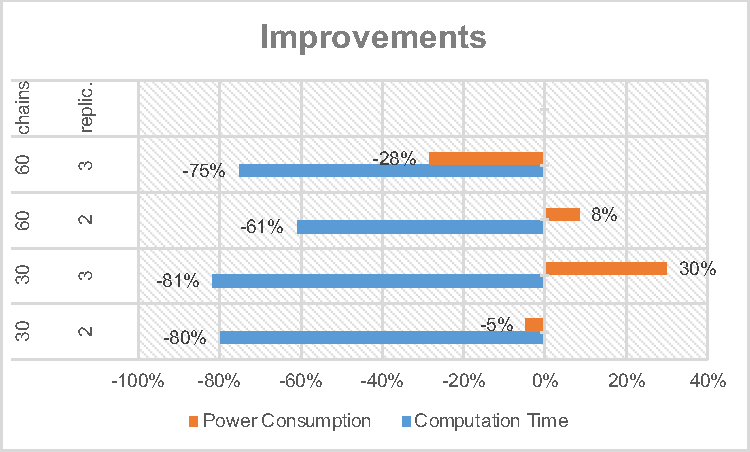
\includegraphics[width=0.7\linewidth]{images/chains_replication_improvements}
	\caption{Effect of approximate algorithm over delay calculations with replication.}
	\label{fig_chainsreplicationimprovements}
\end{figure}

\section{Paper Contributions}
Tables~\ref{paper_contribution} shows the peer-reviewed papers and their contribution to the thesis.
% Please add the following required packages to your document preamble:
% \usepackage{booktabs}
\begin{table}[h]
	\begin{tabular}{@{}llllll@{}}
		\toprule
		Paper & Sec\ref{rc_resa} & Sec\ref{rc_resaanalysis}& Sec\ref{rc_sim} & Sec\ref{rc_ilp} & Sec\ref{rc_pso}\\ \midrule
		A & $\times$ &  &  &  &\\
		B & $\times$ & $\times$ &  & & \\
		C &  & $\times$ &  & & \\
		D &  &  & $\times$ &  &\\
		E &  &  &  & $\times$ &\\
		F &  &  &  & $\times$ &$\times$ \\ \bottomrule
	\end{tabular}
\caption{List of the peer-reviewed papers and their contribution to the thesis.}\label{paper_contribution}
\end{table}
\subsection*{Paper A}
ReSA: An ontology-based requirement specification language tailored to automotive systems. Nesredin~Mahmud, Cristina~Seceleanu and Oscar~Ljungkrantz.\textit{In the 10th IEEE International Symposium on Industrial Embedded Systems (SIES)(pp. 1-10). IEEE, 2015}.\label{lbl_resa}\\[6pt]
\textbf{Abstract:} \textit{Automotive systems are developed using multi-leveled architectural abstractions in an attempt to manage the increasing complexity and criticality of automotive functions. Consequently, well-structured and unambiguously specified requirements are needed on all levels of abstraction, in order to enable early detection of possible design errors. However, automotive industry often relies on requirements specified in ambiguous natural language, sometimes in large and incomprehensible documents. Semi-formal requirements specification approaches (e.g., requirement boilerplates, pattern-based specifications, etc.) aim to reduce requirements ambiguity, without altering their readability and expressiveness. Nevertheless, such approaches do not offer support for specifying requirements in terms of multi-leveled architectural concepts, nor do they provide means for early-stage rigorous analysis of the specified requirements. In this paper, we propose a language, called ReSA, which allows requirements specification at various levels of abstraction, modeled in the architectural language of EAST-ADL. ReSA uses an automotive systems' ontology that offers typing and syntactic axioms for the specification. Besides enforcing structure and more rigor in specifying requirements, our approach enables checking refinement as well as consistency of requirements, by proving ordinary boolean implications. To illustrate ReSA's applicability, we show how to specify some requirements of the Adjustable Speed Limiter, which is a complex, safety-critical Volvo Trucks user function.}\\[6pt]
\textbf{Personal Contributions: }I was the main driver of the paper. I developed the ReSA language including its syntax and semantics, and Cristina Seceleanu proposed a consistency analysis technique besides giving useful comments and ideas on the design of the language. Oscar Ljungkrantz provided useful materials from VGTT that were eventually analyzed for the language development, and gave feedback on the language design and implementation from an industrial viewpoint.\\
\textbf{Status:} Published

\subsection*{Paper B}
ReSA tool: Structured requirements specification and SAT-based consistency-checking. Nesredin~Mahmud, Cristina~Seceleanu and Oscar~Ljungkrantz. \textit{In the 2016 Federated Conference on Computer Science and Information Systems (FedCSIS)(pp. 1737-1746). IEEE, 2016.}\label{lbl_resatool}\\[6pt]
\textbf{Abstract:} \textit{Most industrial embedded systems requirements are
	specified in natural language, hence they can sometimes be
		ambiguous and error-prone. Moreover, employing an early-stage
		model-based incremental system development using multiple
		levels of abstraction, for instance via architectural languages
		such as EAST-ADL, calls for different granularity requirements
		specifications described with abstraction-specific concepts that
		reflect the respective abstraction level effectively.
		In this paper, we propose a toolchain for structured requirements
		specification in the ReSA language, which scales to multiple
		EAST-ADL levels of abstraction. Furthermore, we introduce
		a consistency function that is seamlessly integrated into the
		specification toolchain, for the automatic analysis of requirements
		logical consistency prior to their temporal logic formalization
		for full formal verification. The consistency check subsumes
		two parts: (i) transforming ReSA requirements specification into
		boolean expressions, and (ii) checking the consistency of the
		resulting boolean expressions by solving the satisfiability of their
		conjunction with the Z3 SMT solver. For validation, we apply
		the ReSA toolchain on an industrial vehicle speed control system,
		namely the Adjustable Speed Limiter.}\\[6pt]%abstract
	\textbf{Personal Contributions: }I was the main driver of the paper. I developed the ReSA toolchain that consists of the editor and the consistency checker including the integration with the Z3 SAT solver in the backend. Cristina Seceleanu formulated the consistency checking and together with Oscar Ljungkrantz, they contributed to the paper with useful comments and ideas.\\
		\textbf{Status: }Published

\subsection*{Paper C}
	Specification and semantic analysis of embedded systems requirements: From description logic to temporal logic. Nesredin~Mahmud, Cristina~Seceleanu and Oscar~Ljungkrantz. \textit{In the International Conference on Software Engineering and Formal Methods (SEFM)(pp. 332-348). Springer, Cham, 2017.}\label{lbl_resadl}\\[6pt]%authors
	\textbf{Abstract:} \textit{Due to the increasing complexity of embedded systems, early detection of software/hardware errors has become desirable. In this context, effective yet flexible specification methods that support rigorous analysis of embedded systems requirements are needed. Current specification methods such as pattern-based, boilerplates normally lack meta-models for extensibility and flexibility. In contrast, formal specification languages, like temporal logic, Z, etc., enable rigorous analysis, however, they usually are too mathematical and difficult to comprehend by average software engineers. In this paper, we propose a specification representation of requirements, which considers thematic roles and domain knowledge, enabling deep semantic analysis. The specification is complemented by our constrained natural language specification framework, ReSA, which acts as the interface to the representation. The representation that we propose is encoded in description logic, which is a decidable and computationally-tractable ontology language. By employing the ontology reasoner, Hermit, we check for consistency and completeness of requirements. Moreover, we propose an automatic transformation of the ontology-based specifications into Timed Computation Tree Logic formulas, to be used further in model checking embedded systems.}\\[6pt]%abstract
	\textbf{Personal Contributions:} I was the main driver of the language. I developed the ReSA language semantics using event-base approach, which is encoded in description logic. Cristina~Seceleanu and Ljungkrantz~Oscar provided with useful ideas and comments.\\
	\textbf{Status:} Published

\subsection*{Paper D}
SIMPPAAL - A Framework For Statistical Model Checking of Industrial Simulink Models. Predrag~Filipovikj, Nesredin~Mahmud, Raluca~Marinescu, Cristina~Seceleanu, Oscar~Ljungkrantz and Henrik~L\"{o}nn. \textit{Submitted to ACM Transactions on Software Engineering and Methodology (TOSEM).}\label{lbl_simulink_ilp}
\\[3pt]{\footnotesize This article is an extended version of the following conference paper:
     Simulink to UPPAAL Statistical Model Checker: Analyzing Automotive Industrial Systems.
Predrag Filipovikj, Nesredin Mahmud, Raluca Marinescu, Cristina Seceleanu, Oscar Ljungkrantz, Henrik L{\"o}nn. In Proceedings of the 21st International
Symposium on Formal Methods (FM2016), pages 748-756. Limassol, Cyprus. Springer, LNCS, November 2016. Revisions required. }\\[6pt]%authors
	\noindent \textbf{Abstract:} \textit{The evolution of automotive systems has been rapid. Nowadays, electronic brains control dozens of functions in vehicles, like
		braking, cruising, etc. Model-based design approaches, in environments such as MATLAB Simulink, seem to help in addressing
		the ever-increasing need to enhance quality, and manage complexity, by supporting functional design from a set of block
		libraries, which can be simulated and analyzed for hidden errors, but also used for code generation. For this reason, providing
		assurance that Simulink models fulfill given functional and timing requirements is desirable. In this paper, we propose a
		pattern-based, execution-order preserving automatic transformation of atomic and composite Simulink blocks into stochastic
		timed automata that can then be formally analyzed with Uppaal Statistical Model Checker (Uppaal SMC). To enable this, we
		first define the formal syntax and semantics of Simulink blocks and their composition, and show that the transformation is
		provably correct for a certain class of Simulink models. Our method is supported by the SIMPPAAL tool, which we introduce
		and apply on two industrial Simulink models, a prototype called the Brake-by-Wire and an operational Adjustable Speed
		Limiter system. This work enables the formal analysis of industrial Simulink models, by automatically generating stochastic
		timed automata counterparts.}\\[6pt]%abstract
	\textbf{Personal Contributions: } The three co-authors contributed equally to writing the paper. Technically, I equally contributed with proposing the pattern-based semantics of Simulink blocks, together with Predrag Filipovikj. I introduced a mechanism to enforce the execution order of the blocks using inter-arrival times. Predrag implemented the flattening algorithm and the tool for the automatic transformation of Simulink models into a network of timed automata with stochastic semantics. Raluca Marinescu contributed with analyzing the BBW system, Cristina Seceleanu contributed with defining the methodology, and with useful ideas and comments. Guillermo Rodriguez-Navas wrote the related work section. The industrial coauthors provided the use cases and commented on the final draft.\\
	\noindent\textbf{Status:} Revisions required. 

\subsection*{Paper E}
Power-aware Allocation of Fault-tolerant Multirate AUTOSAR Applications.
     Nesredin~Mahmud, Guillermo~Rodriguez-Navas, Hamid~Faragardi, Saad~Mubeen and Cristina~Seceleanu. \textit{In the 25th Asia-Pacific Software Engineering Conference (APSEC'18). IEEE.}  
     \label{lbl_softwareallocation_ilp}
\\[6pt]%authors
\textbf{Abstract:} \textit{The growing complexity of automotive functionality has attracted revolutionary computing architectures such as mixed-criticality design, which enables effective consolidation of software applications with different criticality on a shared execution platform. Mixed-critical design that is required to satisfy end-to-end timing and reliability specifications should consider power-efficient software design in order to accommodate more and more functionality. Due to the recursive and exhaustive nature of the real-time and reliability analysis, exact methods, e.g., branch and bound, dynamic programming, are prohibitively expensive. We propose hybrid particle-swarm optimization algorithms based on differential evolution and hill-climbing algorithms to minimize power consumption of the safety-critical software, which have end-to-end timing and reliability requirements, on a network of heterogeneous computing units. The optimization approach employs fault tolerance to maximize reliability of the software applications subsequently meet the reliability requirements. Our proposed integrated software-allocation approach is evaluated using a range of synthetic software applications based a real-world automotive benchmark. The evaluation makes comparative analysis of the differential evolution, particle-swarm optimization, integer-linear programming and hybrid particle-swarm optimization algorithms. The results show that the hybrid algorithms based on the hill-climbing algorithms outperform the rest of the meta-heuristic algorithms, in particular, the stochastic version of the hill-climbing algorithm scales well in large software allocation optimization problems while its overall optimality performance can be deemed acceptable.
}\\[6pt]%abstract
\textbf{My Contributions: } I was the main driver of the paper. I developed the system model with the guidance of the co-authors, and formulated the optimization problem with the guidance of Hamid~Faragardi, implemented the the problem in Java, and collected and analyzed the experimental results. The co-authors gave writing updates, useful ideas and comments on the paper, and specifically: Guillermo~Rodriguez-Navas on reliability analysis, Hamid~Faragardi on optimization, Saad~Mubeen on the timing analysis and Cristina~Seceleanu on the objective function and constraints.\\
\textbf{Status:} Published

\subsection*{Paper F}
Optimized Allocation of Fault-tolerant Embedded Software with End-to-end Timing Constraints.	\textit{M\"{a}lardalen Real-time Research Center Technical Report (MRTC), ISRN MDH-MRTC-325/2019-1-SE, 2019}. Submitted to Elsevier Journal of Systems Architecture (JSA).\\[6pt]%authors
\textbf{Abstract:} \textit{It is desirable to optimize power consumption of distributed safety-critical software that realize fault tolerance and maximize reliability as a result, to support the increasing complexity of software functionality in safety-critical embedded systems. Likewise, safety-critical applications that are required to meet end-to-end timing constraints may require additional computing resources. In this paper, we propose a scalable software-to-hardware allocation based on hybrid particle-swarm optimization with hill-climbing and differential algorithms to efficiently map software components to a network of heterogeneous computing nodes while meeting the timing and reliability constraints. The approach assumes fixed-priority preemptive scheduling, and delay analysis that value freshness of data, which is typical in control software applications.
Our proposed solution is evaluated on a range of software applications, which are synthesized from a real-world automotive AUTOSAR benchmark. The evaluation makes comparative analysis of the different algorithms, and a solution based on integer-linear programming, which is an exact method. The results show that the hybrid with the hill-climbing algorithms return very close solutions to the exact method and outperformed the hybrid with the differential algorithm, though consumes more time. The hybrid with the stochastic hill-climbing algorithm scales better and its optimality can be deemed acceptable.}\\[6pt]%abstract
\textbf{Personal Contributions: } I was the main driver of the paper. I developed the system model with the guidance of the co-authors, and formulated the optimization problem with the guidance of Hamid~Faragardi, implemented the the problem in Java, and collected and analyzed the experimental results. The co-authors gave writing updates, useful ideas and comments on the paper, and specifically: Guillermo~Rodriguez-Navas on reliability analysis, Hamid~Faragardi on optimization, Saad~Mubeen on the timing analysis and Cristina~Seceleanu on the objective function and constraints. \\%my contribution
\textbf{Status:} Submitted to Journal of System Architecture (JSA), Elsevier Journals.\\
